\chapter{Several Variables and Partial Derivatives} \label{pd:chapter}

%%%%%%%%%%%%%%%%%%%%%%%%%%%%%%%%%%%%%%%%%%%%%%%%%%%%%%%%%%%%%%%%%%%%%%%%%%%%%%

\section{Vector spaces, linear mappings, and convexity}
\label{sec:vectorspaces}

\sectionnotes{3 lectures}

\subsection{Vector spaces}

The euclidean space $\R^n$ has already made an appearance in the metric
space chapter.  In this chapter, we extend the differential calculus
we created for one variable to several variables.  The key idea in
differential calculus is to approximate differentiable functions by linear
functions (approximating the graph by a straight line).
In several variables, we must introduce a little bit of linear
algebra before we can move on.
We start with vector spaces and linear mappings of vector spaces.

While it is common to use $\vec{v}$ or the bold
$\mathbf{v}$ for elements of $\R^n$,
especially in the applied sciences,
we use just plain old $v$, which is common in mathematics.
That is, $v \in \R^n$ is a \emph{\myindex{vector}}, which means 
$v = (v_1,v_2,\ldots,v_n)$\glsadd{not:vector} is an $n$-tuple of
real numbers.\footnote{Subscripts are used for many purposes,
so sometimes we may have several vectors that may also
be identified by subscript, such as a finite or infinite sequence of
vectors $y_1,y_2,\ldots$.}
It is common to write and treat vectors as
\emph{\myindex{column vectors}}, that is, $n$-by-$1$ matrices:
\glsadd{not:vectorcol}
\begin{equation*}
v =
(v_1,v_2,\ldots,v_n) =
{ \left[
\begin{smallmatrix}
v_1 \\ v_2 \\ \vdots \\ v_n
\end{smallmatrix}
\right]
}
\end{equation*}
We do so when convenient.
We call real numbers
\emph{\myindex{scalars}} to distinguish them from vectors.

We often think of vectors as a direction and a magnitude and draw the
vector as an arrow.  The vector $(v_1,v_2,\ldots,v_n)$ is represented
by an arrow from the origin to the point $(v_1,v_2,\ldots,v_n)$.
When we think of vectors as arrows, they are
not based at the origin necessarily; a vector is simply the direction and
the magnitude, and it does not know where it starts.
There is a natural algebraic structure when thinking of vectors as arrows.
We can add vectors as arrows by following one vector and then the other.
And we can take scalar multiples of vectors as arrows by rescaling
the magnitude.  See \figureref{fig:vecasarrow}.
\begin{myfigureht}
\subimport*{figures/}{vecasarrow.pdf_t}
\caption{Vector as an arrow in $\R^2$, and the meaning of addition and
scalar multiplication.\label{fig:vecasarrow}}
\end{myfigureht}

Each vector also represents a point in $\R^n$.  Usually, we think of $v \in \R^n$
as a point if we are thinking of $\R^n$ as a metric space, and we think of
it as an arrow if we think of the so-called \emph{vector space structure} on
$\R^n$ (addition and scalar multiplication).
Let us define the abstract notion of a vector space, as there
are many other vector spaces than just $\R^n$.

\begin{defn}
Let $X$ be a set together with
the operations of addition, $+ \colon X \times X \to X$,
and multiplication, $\cdot \colon \R \times X \to X$, (we usually write $ax$ instead of $a
\cdot x$).  $X$ is called a \emph{\myindex{vector space}} (or a
\emph{\myindex{real vector space}})
if the following conditions are satisfied:
\begin{enumerate}[(i)]
\item
%mbxSTARTIGNORE
\makebox[2.15in][l]{(Addition is associative)}
%mbxENDIGNORE
%mbxlatex (Addition is associative) \quad
If $u, v, w \in X$, then $u+(v+w) = (u+v)+w$.
\item
%mbxSTARTIGNORE
\makebox[2.15in][l]{(Addition is commutative)}
%mbxENDIGNORE
%mbxlatex (Addition is commutative) \quad
If $u, v \in X$, then $u+v = v+u$.
\item \label{vecspacedefn:addidentity}
%mbxSTARTIGNORE
\makebox[2.15in][l]{(Additive identity)}
%mbxENDIGNORE
%mbxlatex (Additive identity) \quad
There is a $0 \in X$ such that $v+0=v$ for all $v \in X$.
\item \label{vecspacedefn:addinverse}
%mbxSTARTIGNORE
\makebox[2.15in][l]{(Additive inverse)}
%mbxENDIGNORE
%mbxlatex (Additive inverse) \quad
For each $v \in X$, there is a $-v \in X$,
such that $v+(-v)=0$.
\item
%mbxSTARTIGNORE
\makebox[2.15in][l]{(Distributive law)}
%mbxENDIGNORE
%mbxlatex (Distributive law) \quad
If $a \in \R$, $u,v \in X$, then
$a(u+v) = au+av$.
\item
%mbxSTARTIGNORE
\makebox[2.15in][l]{(Distributive law)}
%mbxENDIGNORE
%mbxlatex (Distributive law) \quad
If $a,b \in \R$, $v \in X$, then
$(a+b)v = av+bv$.
\item
%mbxSTARTIGNORE
\makebox[2.15in][l]{(Multiplication is associative)}
%mbxENDIGNORE
%mbxlatex (Multiplication is associative) \quad
If $a,b \in \R$, $v \in X$, then
$(ab)v = a(bv)$.
\item
%mbxSTARTIGNORE
\makebox[2.15in][l]{(Multiplicative identity)}
%mbxENDIGNORE
%mbxlatex (Multiplicative identity) \quad
$1v = v$ for all $v \in X$.
\end{enumerate}
Elements of a vector space are usually called \emph{vectors},
even if they
are not elements of $\R^n$ (vectors in the \myquote{traditional} sense).
%
If $Y \subset X$ is a subset that is a vector space itself using the same
operations, then $Y$ is called a \emph{\myindex{subspace}} or
a \emph{\myindex{vector subspace}} of $X$.
\end{defn}

Multiplication by scalars works as one would expect.
For example, $2v = (1+1)v = 1v + 1v = v+v$, similarly $3v = v+v+v$, and
so on.  
One particular fact we often use is that $0 v = 0$, where
the zero on the left is $0 \in \R$ and the zero on the right is $0 \in X$.
To see this, start with
$0v = (0+0)v = 0v + 0v$, and add $-(0v)$ to both sides
to obtain $0 = 0v$.  Similarly, $-v = (-1)v$, which follows by
$(-1)v+v = (-1)v + 1v = (-1+1)v = 0v = 0$.
Such algebraic facts which follow quickly from the definition will be taken
for granted from now on.

\begin{example}
The set $\R^n$ is a vector space, addition
and multiplication by a scalar is done componentwise:
If $a \in \R$, $v = (v_1,v_2,\ldots,v_n) \in \R^n$, and $w =
(w_1,w_2,\ldots,w_n) \in \R^n$, then
\begin{align*}
& v+w \coloneqq
(v_1,v_2,\ldots,v_n) +
(w_1,w_2,\ldots,w_n) 
=
(v_1+w_1,v_2+w_2,\ldots,v_n+w_n) , \\
& a v \coloneqq
a (v_1,v_2,\ldots,v_n) =
(a v_1, a v_2,\ldots, a v_n) .
\end{align*}
\end{example}

We will mostly deal with \myquote{finite-dimensional} vector spaces that can
be regarded as subsets of $\R^n$, but other vector spaces are useful in
analysis.
It is better to think of even such simpler
vector spaces abstractly abstract notion rather than as $\R^n$.

\begin{example}
A trivial example of a vector space is
$X \coloneqq \{ 0 \}$.  The operations are defined in the obvious way:
$0 + 0 \coloneqq 0$ and $a0 \coloneqq 0$.  A zero vector must always exist,
so all vector spaces are nonempty sets, and this $X$ is the smallest
possible vector space.
\end{example}

\begin{example}
The space $C([0,1],\R)$ of continuous functions on the interval $[0,1]$
is a vector space.  For two functions $f$ and $g$ in $C([0,1],\R)$ and
$a \in \R$, we make the obvious definitions of $f+g$ and $af$:
\begin{equation*}
(f+g)(x) \coloneqq f(x) + g(x), \qquad (af) (x) \coloneqq a\bigl(f(x)\bigr) .
\end{equation*}
The 0 is the function that is identically zero.  We leave it as an exercise
to check that all the vector space conditions are satisfied.
The space $C^1([0,1],\R)$ of continuously differentiable functions is
a subspace of $C([0,1],\R)$.
\end{example}

\begin{example}
The space of polynomials $c_0 + c_1 t + c_2 t^2 + \cdots + c_m t^m$
(of arbitrary degree~$m$) is a vector space,
denoted by $\R[t]$\glsadd{not:realpoly} (coefficients are real and
the variable is $t$).  The operations are defined in the same way as for
functions above.
Suppose there are
two polynomials, one of degree $m$ and one of degree $n$.  Assume $n
\geq m$ for simplicity.  Then
\begin{multline*}
(c_0 + c_1 t + c_2 t^2 + \cdots + c_m t^m)
+
(d_0 + d_1 t + d_2 t^2 + \cdots + d_n t^n)
= \\
(c_0+d_0) + (c_1+d_1) t + (c_2 + d_2) t^2 + \cdots + (c_m+d_m) t^m
+ d_{m+1} t^{m+1} + \cdots + d_n t^n
\end{multline*}
and
\begin{equation*}
a(c_0 + c_1 t + c_2 t^2 + \cdots + c_m t^m)
=
(ac_0) + (ac_1) t + (ac_2) t^2 + \cdots + (ac_m) t^m  .
\end{equation*}
Despite what it looks like, $\R[t]$ is not equivalent to $\R^n$ for any $n$.  In
particular, it is not \myquote{finite-dimensional.}  We will make this notion
precise in just a little bit.  One can make a
finite-dimensional vector subspace by restricting the degree.  For example,
if $\sP_n$ is the set of polynomials of degree $n$ or less,
then $\sP_n$ is a finite-dimensional vector space, and we could 
identify it with $\R^{n+1}$.

Above, the variable $t$ is really just a formal placeholder.
By setting $t$ equal to a real number, we obtain a function.
So the space $\R[t]$ can be thought of as a subspace of $C(\R,\R)$.
If we restrict the range of $t$ to $[0,1]$, $\R[t]$ can be identified with
a subspace of $C([0,1],\R)$.
\end{example}

\begin{prop}
For $S \subset X$ to be a vector subspace
of a vector space $X$, we only need to check:
%If $X$ is a vector space, for $S \subset X$
%to be a vector subspace, we only need to check
\begin{enumerate}[1)]
\item
$0 \in S$.
\item
$S$ is closed under addition: If $x,y \in S$, then $x+y \in S$.
\item
$S$ is closed under scalar multiplication:
If $x \in S$ and $a \in \R$, then $ax \in S$.
\end{enumerate}
\end{prop}

Items 2) and 3)
ensure that addition and scalar multiplication are indeed defined on~$S$.
Item 1) is required
to fulfill item \ref{vecspacedefn:addidentity} from the definition of vector
space.  Existence
of additive inverse $-v$, item \ref{vecspacedefn:addinverse},
follows because $-v = (-1)v$ and item 3) says that
$-v \in S$ if $v \in S$.  All other properties are certain equalities
that are already satisfied in $X$ and thus must be satisfied in a subset.

\medskip

It is possible to use other fields than $\R$ in the definition
(for example, it is common to use the complex numbers $\C$),
but let us stick with
the real numbers\footnote{If you want a very funky vector space over a different field,
$\R$ itself is a vector space over the field $\Q$.}.

\subsection{Linear combinations and dimension}

\begin{defn}
Suppose $X$ is a vector space,
$x_1, x_2, \ldots, x_m \in X$ are vectors, and
$a_1, a_2, \ldots, a_m \in \R$ are scalars.  Then
\begin{equation*}
a_1 x_1 + 
a_2 x_2 +  \cdots
+ a_m x_m
\end{equation*}
is called a \emph{\myindex{linear combination}} of the vectors $x_1, x_2,
\ldots, x_m$.

For a subset $Y \subset X$, let $\spn(Y)$,\glsadd{not:span}
or the \emph{\myindex{span}} of $Y$,
be the set of all linear combinations of all finite subsets of $Y$.
We say $Y$ \emph{spans} $\spn(Y)$.
By convention, define $\spn(\emptyset) \coloneqq \{ 0 \}$.
\end{defn}

\begin{example}
Let $Y \coloneqq \bigl\{ (1,1) \bigr\} \subset \R^2$.  Then
\begin{equation*}
\spn(Y)
=
\bigl\{ (x,x) \in \R^2 : x \in \R \bigr\} .
\end{equation*}
That is, $\spn(Y)$ is the line through the origin and the point $(1,1)$.
\end{example}

\begin{example} \label{example:vecspr2span}
Let $Y \coloneqq \bigl\{ (1,1), (0,1) \bigr\} \subset \R^2$.  Then
\begin{equation*}
\spn(Y)
=
\R^2 ,
\end{equation*}
as every point $(x,y) \in \R^2$ can be written as
a linear combination
\begin{equation*}
(x,y) = x (1,1) + (y-x) (0,1) .
\end{equation*}
\end{example}

\begin{example}
Let $Y \coloneqq \{ 1, t, t^2, t^3, \ldots \} \subset \R[t]$, and
$E \coloneqq \{ 1, t^2, t^4, t^6, \ldots \} \subset \R[t]$.
The span of $Y$ is all polynomials,
\begin{equation*}
\spn(Y) = \R[t] .
\end{equation*}
The span of $E$ is the set of polynomials with even powers of $t$ only.
\end{example}

Suppose we have two linear combinations of vectors from $Y$.  One linear
combination uses the vectors $\{ x_1,x_2,\ldots,x_m \}$, and the other uses
$\{ \widetilde{x}_1,\widetilde{x}_2,\ldots,\widetilde{x}_n \}$.  We can write
their sum using vectors from the union
$\{ x_1,x_2,\ldots,x_m \} \cup
\{ \widetilde{x}_1,\widetilde{x}_2,\ldots,\widetilde{x}_n \}$:
\begin{multline*}
(a_1 x_1 + 
a_2 x_2 +  \cdots
+ a_m x_m)
+
(b_1 \widetilde{x}_1 + 
b_2 \widetilde{x}_2 +  \cdots
+ b_n \widetilde{x}_n)
\\
=
a_1 x_1 + 
a_2 x_2 +  \cdots
+ a_m x_m
+
b_1 \widetilde{x}_1 + 
b_2 \widetilde{x}_2 +  \cdots
+ b_n \widetilde{x}_n .
\end{multline*}
So the sum is also a linear combination of vectors from~$Y$.
Similarly,
a scalar multiple of a linear combination of vectors from~$Y$
is a linear combination of vectors from~$Y$:
\begin{equation*}
b (a_1 x_1 + 
a_2 x_2 +  \cdots
+ a_m x_m)
=
b a_1  x_1 + 
b a_2 x_2 +  \cdots
+ b a_m x_m .
\end{equation*}
Finally, $0 \in \spn(Y)$; if $Y$ is nonempty, $0 = 0 v$ for some $v \in Y$.
We have proved the following proposition.

\begin{prop}
Let $X$ be a vector space and $Y \subset X$ is a subset.
Then the set $\spn(Y)$ is a vector subspace of $X$.
\end{prop}

Every linear combination of elements in a subspace is an element of that
subspace.  So $\spn(Y)$ is the smallest subspace that contains $Y$.
In particular,
if $Y$ is already a vector subspace, then $\spn(Y) = Y$.

\begin{defn}
A set of vectors $\{ x_1, x_2, \ldots, x_m \} \subset X$ is 
\emph{\myindex{linearly independent}}\footnote{%
For an infinite set $Y \subset X$, we say $Y$ is linearly
independent if every finite subset of $Y$ is linearly independent
in the sense given.
However, this situation only comes up in infinitely many dimensions.}
if the equation
\begin{equation} \label{eq:lincomb}
a_1 x_1 + a_2 x_2 + \cdots + a_m x_m = 0
\end{equation}
has only the trivial solution $a_1 = a_2 = \cdots = a_m = 0$.
By convention, $\emptyset$ is linearly independent.
A set that is not linearly independent is
\emph{\myindex{linearly dependent}}.
%
A linearly independent set of vectors $B \subset X$ such that
$\spn(B) = X$ 
is called a \emph{\myindex{basis}} of $X$.
We generally consider the basis as not just a set, but as
an ordered $m$-tuple:
$x_1,x_2,\ldots,x_m$.

Suppose $d$ is largest integer for which $X$ contains a set of
$d$ linearly independent vectors.  We then say $d$ is
the \emph{\myindex{dimension}} of $X$,
and we write $\dim \, X \coloneqq d$.
If $X$ contains a set of $d$ linearly independent vectors 
for arbitrarily large $d$, we say
$X$ is infinite-dimensional and write $\dim \, X \coloneqq \infty$.
%
For the trivial vector space $\{ 0 \}$, we define $\dim \, \{ 0 \} \coloneqq 0$.
\end{defn}

A subset of a linearly independent set is clearly linearly independent.
So if a set contains $d$ linearly independent vectors, it also contains a
set of $m$ linearly independent vectors for all $m \leq d$.
Moreover, if a set does not have $d+1$
linearly independent vectors, no set of more than $d+1$ vectors is linearly
independent.
So $X$ is of dimension is $d$ if there
is a set of $d$ linearly independent vectors, but no
set of $d+1$ vectors is linearly independent.

No element of a linearly independent set can be zero,
and a set with one nonzero element is always linearly independent.
In particular, $\{ 0 \}$ is the only vector space of dimension $0$.
Every other vector space has a positive dimension
or is infinite-dimensional.
As the empty set is linearly independent, it is a basis
of $\{ 0 \}$.

As an example, the
set $Y$ of the two vectors in
\exampleref{example:vecspr2span} is a basis of $\R^2$, and so
$\dim \, \R^2 \geq 2$.
We will see in a moment that every vector subspace of $\R^n$
has a finite dimension, and that dimension is less than or equal to $n$.
So every set of 3 vectors in $\R^2$ is linearly dependent, and
$\dim \, \R^2 = 2$.

If a set is linearly dependent, then one of the
vectors is a linear combination of the others.
In \eqref{eq:lincomb},
if $a_k \not= 0$, then we solve for $x_k$:
\begin{equation*}
x_k = \frac{-a_1}{a_k} x_1 + \cdots + 
\frac{-a_{k-1}}{a_k} x_{k-1} +
\frac{-a_{k+1}}{a_k} x_{k+1} +
\cdots + 
\frac{-a_m}{a_m} x_m .
\end{equation*}
The vector $x_k$ has at least two different representations
as linear combinations of the vectors $\{ x_1,x_2,\ldots,x_m \}$. The one above and
$x_k$ itself. 
For instance, the set $\bigl\{ (0,1), (2,3), (5,0) \bigr\}$ in $\R^2$ is linearly dependent:
\begin{equation*}
3(0,1) - (2,3) + 2(1,0) = 0 ,
\qquad \text{so} \qquad
(2,3) = 3(0,1) + 2(1,0) .
\end{equation*}

\begin{prop}
Suppose a vector space $X$ has basis 
$B = \{ x_1, x_2, \ldots, x_n \}$.  Then
every $y \in X$ has a unique representation of the form
\begin{equation*}
y = \sum_{k=1}^n a_k \, x_k
\end{equation*}
for some scalars $a_1, a_2, \ldots, a_n$.
\end{prop}

\begin{proof}
As $X$ is the span of $B$,
every $y \in X$ is a linear combination of elements of $B$.
Suppose
\begin{equation*}
y = \sum_{k=1}^n a_k \, x_k = \sum_{k=1}^n b_k \, x_k .
\end{equation*}
Then
\begin{equation*}
\sum_{k=1}^n (a_k-b_k) x_k = 0 .
\end{equation*}
By linear independence of the basis, $a_k = b_k$ for all $k$, and so
the representation is unique.
\end{proof}

For $\R^n$,
we define
the \emph{\myindex{standard basis}} of $\R^n$:\glsadd{not:standardbasis}
\begin{equation*}
e_1 \coloneqq (1,0,0,\ldots,0) , \quad
e_2 \coloneqq (0,1,0,\ldots,0) , \quad \ldots, \quad
e_n \coloneqq (0,0,0,\ldots,1) ,
\end{equation*}
We use the same letters $e_k$ for any $\R^n$, and
which space $\R^n$ we are working in is understood from context.
A direct computation shows that $\{ e_1, e_2, \ldots, e_n \}$ really is
a basis of $\R^n$; it spans $\R^n$ and is
linearly independent.  In fact,
\begin{equation*}
a = (a_1,a_2,\ldots,a_n) = \sum_{k=1}^n a_k \, e_k .
\end{equation*}

\begin{prop} \label{mv:dimprop}
\pagebreak[2]
Let $X$ be a vector space and $d$ a nonnegative integer.
\begin{enumerate}[(i)]
\item \label{mv:dimprop:i}
If $X$ is spanned by $d$ vectors, then $\dim \, X \leq d$.
\item \label{mv:dimprop:ii}
If $T$ is a linearly independent set and
$v \in X \setminus \spn (T)$, then
$T \cup \{ v \}$ is linearly independent.
\item \label{mv:dimprop:iii}
$\dim \, X = d$ if and only if $X$ has a basis of $d$
vectors.
In particular, $\dim \, \R^n = n$.
\item \label{mv:dimprop:iv}
If $Y \subset X$ is a vector subspace and $\dim \, X = d$,
then $\dim \, Y \leq d$.
\item \label{mv:dimprop:v}
If $\dim \, X = d$ and a set $T$ of $d$ vectors spans $X$,
then $T$ is linearly independent.
\item \label{mv:dimprop:vi}
If $\dim \, X = d$ and a set $T$ of $m$ vectors is
linearly independent, then there is a set $S$ of $d-m$
vectors such that $T \cup S$ is a basis of $X$.
\end{enumerate}
\end{prop}

In particular, the last item says that if $\dim X = d$ and $T$ is
a set of $d$ linearly independent vectors, then $T$ spans $X$.
Another thing to note is that item \ref{mv:dimprop:iii} implies that every
basis of a finite dimensional vector space has the same number of elements.

\begin{proof}
All statements hold trivially when $d=0$, so assume $d \geq 1$.

We start with \ref{mv:dimprop:i}.
Suppose $S \coloneqq \{ x_1 , x_2, \ldots, x_d \}$ spans $X$, and
$T \coloneqq \{ y_1, y_2, \ldots, y_m \}$ is a linearly independent
subset of $X$.  We wish to show that $m \leq d$.
As $S$ spans $X$,
write
\begin{equation*}
y_1 = \sum_{k=1}^d a_{k,1} x_k ,
\end{equation*}
for some numbers $a_{1,1},a_{2,1},\ldots,a_{d,1}$.
One of the
$a_{k,1}$ is nonzero, otherwise $y_1$ would be zero.
Without loss of generality, suppose $a_{1,1} \not= 0$.  Solve
\begin{equation*}
x_1 = \frac{1}{a_{1,1}} y_1 - \sum_{k=2}^d \frac{a_{k,1}}{a_{1,1}} x_k .
\end{equation*}
In particular, $\{ y_1 , x_2, \ldots, x_d \}$ spans $X$, since $x_1$ can be
obtained from $\{ y_1 , x_2, \ldots, x_d \}$.  Therefore, there are some numbers
for some numbers $a_{1,2},a_{2,2},\ldots,a_{d,2}$, such that
\begin{equation*}
y_2 = a_{1,2} y_1 + \sum_{k=2}^d a_{k,2} x_k .
\end{equation*}
As $T$ is linearly independent---and so $\{ y_1, y_2 \}$ is linearly
independent---one of the $a_{k,2}$
for $k \geq 2$ must be nonzero.  Without loss of generality suppose 
$a_{2,2} \not= 0$.  Solve
\begin{equation*}
x_2 = \frac{1}{a_{2,2}} y_2 - \frac{a_{1,2}}{a_{2,2}} y_1 - \sum_{k=3}^d
\frac{a_{k,2}}{a_{2,2}} x_k .
\avoidbreak
\end{equation*}
In particular,
$\{ y_1 , y_2, x_3, \ldots, x_d \}$ spans $X$.

We continue this procedure.  If $m < d$, we are done.  Suppose
$m \geq d$.
After $d$ steps, we obtain that 
$\{ y_1 , y_2, \ldots, y_d \}$ spans $X$.  Any
other vector $v$ in $X$ is a linear combination of
$\{ y_1 , y_2, \ldots, y_d \}$ and hence cannot be in $T$ as $T$ is
linearly independent.  So $m = d$.

We continue with \ref{mv:dimprop:ii}.
Suppose 
$T = \{x_1,x_2,\ldots,x_m\}$ is linearly independent,
does not span $X$, and $v \in X \setminus \spn (T)$.
Suppose 
$a_1 x_1 + a_2 x_2 + \cdots + a_m x_m + a_{m+1} v = 0$
for some scalars $a_1,a_2,\ldots,a_{m+1}$.
If $a_{m+1} \not=0$, then $v$ would be a linear combination of $T$,
so $a_{m+1} = 0$.  Then, as $T$ is linearly independent, $a_1=a_2=\cdots=a_m = 0$.
So $T \cup \{ v \}$ is linearly independent.

We move to \ref{mv:dimprop:iii}.
If $\dim \, X = d$,
then there must exist some linearly independent set $T$ of $d$ vectors,
and $T$ must span $X$, otherwise we could choose a larger set of linearly
independent vectors via \ref{mv:dimprop:ii}.
So we have a basis of $d$ vectors.
On the other hand, if we have a basis of $d$ vectors,
the dimension is at least $d$ as a basis is linearly independent.
A basis also spans $X$, and so
by \ref{mv:dimprop:i} we know that dimension is at most $d$.
Hence the dimension of $X$ must equal $d$.
The \myquote{in particular} follows by noting that
$\{ e_1, e_2, \ldots, e_n \}$ is a basis of $\R^n$.

To see \ref{mv:dimprop:iv},
suppose $Y \subset X$ is a vector subspace,
where $\dim \, X = d$.  As $X$ cannot contain $d+1$ linearly independent
vectors, neither can $Y$.

For \ref{mv:dimprop:v}, suppose $T$ is a set of $m$ vectors
that is linearly dependent
and spans $X$.
We will show that $m > d$.
One of the
vectors is a linear combination of the others.  If we remove it
from $T$, we obtain a set of $m-1$ vectors that still span $X$.
Hence
$d = \dim \, X \leq m-1$ by~\ref{mv:dimprop:i}.

For \ref{mv:dimprop:vi} suppose $T = \{ x_1, x_2, \ldots, x_m \}$ is
a linearly independent set.  First, $m \leq d$ by definition of dimension.
If $m=d$, the set $T$ must span $X$ as in the proof of \ref{mv:dimprop:iii},
otherwise we could add another vector to $T$.
If $m < d$,  $T$ cannot span $X$ by \ref{mv:dimprop:iii}.
So find $v$ not in the span of~$T$.
Via \ref{mv:dimprop:ii}, the set $T \cup \{ v \}$ is
a linearly independent set of $m+1$ elements.
Therefore, we repeat this procedure $d-m$ times to
find a set of $d$ linearly independent vectors.
Again, they must span $X$, otherwise we could add yet another vector.
\end{proof}

\subsection{Linear mappings}

When $Y \not= \R$,
a function $f \colon X \to Y$ is often called a
\emph{\myindex{mapping}} or a \emph{\myindex{map}}
rather than a \emph{function}.

\begin{defn}
A map $A \colon X \to Y$ of vector spaces $X$ and $Y$
is \emph{\myindex{linear}} (we also say $A$ is a
\emph{\myindex{linear transformation}}\index{transformation, linear}
or a \emph{\myindex{linear operator}}\index{operator, linear})
if for all $a \in \R$ and all $x,y \in X$,
\begin{equation*}
A(a x) = a A(x) \qquad \text{and} \qquad A(x+y) = A(x)+A(y) .
\end{equation*}
We usually write $Ax$ instead of $A(x)$ if $A$ is linear.
If $A$ is one-to-one and onto, then we say $A$ is
\emph{invertible}\index{invertible linear transformation},
and we denote the inverse by $A^{-1}$.
If $A \colon X \to X$ is linear, then we say $A$ is a
\emph{linear operator on $X$}.

We write $L(X,Y)$\glsadd{not:LXY} for the set of linear maps from $X$ to
$Y$, and $L(X)$\glsadd{not:LX} for the set of linear operators on $X$.
If $a \in \R$ and $A,B \in L(X,Y)$, define
the maps $aA$ and $A+B$ by
\begin{equation*}
(aA)(x) \coloneqq aAx ,
\qquad
(A+B)(x) \coloneqq Ax + Bx .
\end{equation*}
If $A \in L(Y,Z)$ and $B \in L(X,Y)$, define the
map $AB \colon X \to Z$ as the composition $A \circ B$,
\begin{equation*}
ABx \coloneqq A(Bx) .
\end{equation*}
Finally, denote by $I \in L(X)$ the \emph{\myindex{identity}}: 
the linear operator such that $Ix = x$ for all $x$.
\end{defn}

\begin{prop} \label{prop:LXYvs}
Let $X$, $Y$, and $Z$ be vector spaces.
\begin{enumerate}[(i)]
\item If $A \in L(X,Y)$, then $A0 = 0$.
\item If $A,B \in L(X,Y)$, then $A+B \in L(X,Y)$.
\item If $A \in L(X,Y)$ and $a \in \R$, then $aA \in L(X,Y)$.
\item If $A \in L(Y,Z)$ and $B \in L(X,Y)$, then $AB \in L(X,Z)$. 
\item If $A \in L(X,Y)$ is invertible, then $A^{-1} \in L(Y,X)$.
\end{enumerate}
\end{prop}

In particular, $L(X,Y)$ is a vector space, where $0 \in L(X,Y)$ is the
linear map that takes everything to $0$.
As $L(X)$ is not only a vector space, but also
admits a product (composition),
it is called an \emph{\myindex{algebra}}.

\begin{proof}
We leave the first four items as a quick exercise,
\exerciseref{exercise:LXYvs}.
Let us prove the last item.
Let $a \in \R$ and $y \in Y$.  As $A$ is onto, then there is an 
$x \in X$ such that $y = Ax$.
As it is also one-to-one, $A^{-1}(Az) = z$ for all $z \in X$.
So
\begin{equation*}
A^{-1}(ay)
=
A^{-1}(aAx)
=
A^{-1}\bigl(A(ax)\bigr)
= ax
= aA^{-1}(y).
\end{equation*}
Similarly, let $y_1,y_2 \in Y$ and $x_1, x_2 \in X$ be such that
$Ax_1 = y_1$ and 
$Ax_2 = y_2$, then
\begin{equation*}
A^{-1}(y_1+y_2)
=
A^{-1}(Ax_1+Ax_2)
=
A^{-1}\bigl(A(x_1+x_2)\bigr)
= x_1+x_2
= A^{-1}(y_1) + A^{-1}(y_2). \qedhere
\end{equation*}
\end{proof}

\begin{prop} \label{mv:lindefonbasis}
If $A \in L(X,Y)$ is linear, then it is completely determined
by its values on a basis of $X$.
Furthermore, if $B$ is a basis of $X$,
then every function $\widetilde{A} \colon B \to Y$ extends to a linear
function $A$ on $X$.
\end{prop}

We only prove this proposition for finite-dimensional spaces, as we do
not need infinite-dimensional spaces.%
\footnote{For infinite-dimensional spaces, the proof is essentially the same, but a
little trickier to write.
Moreover, we haven't even defined what a basis is for
infinite-dimensional spaces.}

\begin{proof}
Let $\{ x_1, x_2, \ldots, x_n \}$ be a basis of $X$, and let 
$y_k \coloneqq A x_k$.  Every $x \in X$ has a unique representation
\begin{equation*}
x = \sum_{k=1}^n b_k \, x_k
\end{equation*}
for some numbers $b_1,b_2,\ldots,b_n$.  By linearity,
\begin{equation*}
Ax = 
A\sum_{k=1}^n b_k x_k
=
\sum_{k=1}^n b_k \, Ax_k
=
\sum_{k=1}^n b_k \, y_k .
\end{equation*}
The \myquote{furthermore} follows by setting $y_k \coloneqq \widetilde{A}(x_k)$,
and then for 
$x = \sum_{k=1}^n b_k \, x_k$,
defining the extension as
$A(x) \coloneqq \sum_{k=1}^n b_k \, y_k$.  The function is well-defined by
uniqueness of the representation of $x$.
We leave it to the reader to check that $A$ is linear.
\end{proof}

The next proposition only works for finite-dimensional vector spaces.
It is a special case of the so-called rank-nullity theorem from linear
algebra.

\begin{prop} \label{mv:prop:lin11onto}
If $X$ is a finite-dimensional vector space and $A \in L(X)$, then $A$ is one-to-one if and only if it is onto.
\end{prop}

\begin{proof}
Let $\{ x_1,x_2,\ldots,x_n \}$ be a basis for $X$.
First suppose $A$ is one-to-one.  Let $c_1,c_2,\ldots,c_n$ be such that
\begin{equation*}
0 =
\sum_{k=1}^n c_k \, Ax_k =
A\sum_{k=1}^n c_k \, x_k 
.
\end{equation*}
As $A$ is one-to-one,
the only vector that is taken to 0 is 0 itself.  
Hence,
\begin{equation*}
0 =
\sum_{k=1}^n c_k \, x_k,
\end{equation*}
and so $c_k = 0$ for all $k$ as $\{ x_1,x_2,\ldots,x_n \}$ is a basis.
So $\{ Ax_1, Ax_2, \ldots, Ax_n \}$ is linearly independent.
By \propref{mv:dimprop}
and the fact that the dimension is $n$, we conclude
$\{ Ax_1, Ax_2, \ldots, Ax_n \}$ spans $X$.  Any point $x \in X$
can be written as
\begin{equation*}
x = \sum_{k=1}^n a_k \, Ax_k =
A\sum_{k=1}^n a_k \, x_k ,
\avoidbreak
\end{equation*}
so $A$ is onto.

For the other direction, suppose $A$ is onto.
Suppose that for some
$c_1,c_2,\ldots,c_n$,
\begin{equation*}
0 = A\sum_{k=1}^n c_k \, x_k =
\sum_{k=1}^n c_k \, Ax_k .
\end{equation*}
As $A$ is determined by the action on the basis,
$\{ Ax_1, Ax_2, \ldots, Ax_n \}$ spans $X$.
So by \propref{mv:dimprop}, the set is linearly independent,
and $c_k = 0$ for all $k$.  In other words, if $Ax = 0$, then $x=0$.
Thus, $A$ is one-to-one:  If $Ax = Ay$, then $A(x-y) = 0$ and so
$x=y$.
\end{proof}

We leave the proof of the next proposition as an exercise.

\begin{prop} \label{prop:LXYfinitedim}
If $X$ and $Y$ are finite-dimensional vector spaces, then $L(X,Y)$
is also finite-dimensional.
\end{prop}

We can identify a finite-dimensional vector
space $X$ of dimension $n$ with $\R^n$, provided we fix a basis
$\{ x_1, x_2, \ldots, x_n \}$ in $X$.  That is, we define a bijective
linear map $A \in L(X,\R^n)$ by
$Ax_k \coloneqq e_k$, where $\{ e_1, e_2, \ldots, e_n \}$ is the standard
basis in $\R^n$.  We have
the correspondence\glsadd{not:mapsto}
\begin{equation*}
\sum_{k=1}^n c_k \, x_k \, \in X
\quad
\overset{A}{\mapsto}
\quad
(c_1,c_2,\ldots,c_n) \, \in \R^n .
\end{equation*}

\subsection{Convexity}

A subset $U$ of a vector space is \emph{\myindex{convex}}
if whenever $x,y \in U$, the line segment from
$x$ to $y$ lies in $U$.  That is, if the \emph{\myindex{convex combination}}
$(1-t)x+ty$ is in $U$ for all $t \in [0,1]$.
We write $[x,y]$ for this line segment.\glsadd{not:segmentinRn}
See \figureref{mv:convexcomb}.

\begin{myfigureht}
\subimport*{figures/}{convexset.pdf_t}
\caption{Convexity.\label{mv:convexcomb}}
\end{myfigureht}

In $\R$, convex sets are precisely the intervals, which are
also precisely the connected sets.
In two or more dimensions
there are lots of nonconvex connected sets.  For example,
the set $\R^2 \setminus \{0\}$ is connected,
but not convex---for any $x \in \R^2 \setminus \{0\}$ where $y \coloneqq -x$,
we find
$(\nicefrac{1}{2})x + (\nicefrac{1}{2})y = 0$, which is not in the set.
Balls (in the standard metric) in $\R^n$ are convex.  It is
a useful enough result to state as a proposition,
but we leave its proof as an exercise.

\begin{prop}
Let $x \in \R^n$ and $r > 0$.  The ball $B(x,r) \subset \R^n$
%(using the standard metric on $\R^n$)
is convex.
\end{prop}

\begin{example}
A convex combination is, in particular, a linear combination.
So every vector subspace $V$ of a vector space $X$ is convex.
\end{example}

\begin{example}
%A somewhat more complicated example is given by the following.
Let $C([0,1],\R)$ be the vector space of continuous real-valued functions on $\R$.
Let $V \subset C([0,1],\R)$ be the set of those $f$ such that
\begin{equation*}
\int_0^1 f(x)\,dx \leq 1 \qquad \text{and} \qquad
f(x) \geq 0 \enspace \text{for all } x \in [0,1] .
\end{equation*}
Then $V$ is convex.  Take $t \in [0,1]$, and note that if $f,g \in V$,
then $(1-t) f(x) + t g(x) \geq 0$ for all $x$.  Furthermore,
\begin{equation*}
\int_0^1 \bigl((1-t)f(x) + t g(x)\bigr) \,dx
=
(1-t) \int_0^1 f(x) \,dx
+ t \int_0^1 g(x) \,dx \leq 1 .
\end{equation*}
Note that $V$ is not a vector subspace of $C([0,1],\R)$.  The function
$f(x) \coloneqq 1$ is in $V$, but $2f$ and $-f$ is not.
\end{example}

\begin{prop} \label{prop:intersectionconvex}
The intersection of two convex sets is convex.  In fact,
if $\{ C_\lambda \}_{\lambda \in I}$ is
an arbitrary collection of convex sets in a vector space, then
\begin{equation*}
C \coloneqq \bigcap_{\lambda \in I} C_\lambda
\qquad \text{is convex.}
\end{equation*}
\end{prop}

\begin{proof}
If $x, y \in C$, then $x,y \in C_\lambda$ for all
$\lambda \in I$, and hence if $t \in [0,1]$, then $(1-t)x + ty \in
C_\lambda$ for all $\lambda \in I$.  Therefore, $(1-t)x + ty \in C$ and $C$
is convex.
\end{proof}

A useful construction using intersections of convex sets is the
\emph{\myindex{convex hull}}.  Given a subset $S$ of a vector
space $X$, define the convex hull of $S$ as the intersection of all convex sets
containing $S$:
\begin{equation*}
\operatorname{co}(S) \coloneqq
\bigcap \{ C \subset X : S \subset C, \text{ and } C \text{ is convex} \} .
\end{equation*}
That is, the convex hull is the smallest convex set containing $S$.  
By \propref{prop:intersectionconvex}, the intersection of convex sets is
convex.
Hence the convex hull is convex.

\begin{example}
The convex hull of $\{ 0, 1 \}$ in $\R$ is $[0,1]$.  Proof:
A convex set containing 0 and 1 must contain $[0,1]$, so
$[0,1] \subset \operatorname{co}(\{0,1\})$.
The set $[0,1]$ is convex and contains $\{0,1\}$, so
$\operatorname{co}(\{0,1\}) \subset [0,1]$.
\end{example}

Linear mappings preserve convex sets.  So in some sense, convex sets are the
right sort of sets when considering linear mappings or changes of
coordinates.

\begin{prop}
Let $X,Y$ be vector spaces, $A \in L(X,Y)$, and let $C \subset X$ be convex.
Then $A(C)$ is convex.
\end{prop}

\begin{proof}
Take two points $p,q \in A(C)$.  Pick $u,v \in C$ such that
$Au = p$ and $Av=q$.  As $C$ is convex, then
$(1-t)u+t v \in C$
for all $t \in [0,1]$, so
\begin{equation*}
(1-t)p+t q 
=
(1-t)Au+tAv
=
A\bigl((1-t)u+tv\bigr)
\in A(C) .  \qedhere
\end{equation*}
\end{proof}


\subsection{Exercises}

\begin{exercise}
Show that in $\R^n$
(with the standard euclidean metric),
for every $x \in \R^n$ and every $r > 0$,
the ball $B(x,r)$ is convex.
\end{exercise}


\begin{exercise}
Verify that $\R^n$ is a vector space.
\end{exercise}

\begin{exercise}
Let $X$ be a vector space.
Prove that a finite set of vectors $\{ x_1,x_2,\ldots,x_n \} \subset X$ 
is linearly independent if and only if for every $k=1,2,\ldots,n$
\begin{equation*}
\spn\bigl( \{ x_1,\ldots,x_{k-1},x_{k+1},\ldots,x_n \}\bigr) \subsetneq
\spn\bigl( \{ x_1,x_2,\ldots,x_n \}\bigr) .
\end{equation*}
That is, the span of the set with one vector removed is strictly smaller.
\end{exercise}

\begin{exercise} \label{exercise:intzerosubspace}
Show that the set $X \subset C([0,1],\R)$ of those functions such 
that $\int_0^1 f = 0$ is a vector subspace.
Compare \exerciseref{exercise:intoneconvex}.
\end{exercise}

\begin{exercise}[Challenging]
Prove $C([0,1],\R)$ is an infinite-dimensional vector space
where the operations are defined in the obvious way:
$s=f+g$ and $m=af$ are defined as
$s(x) \coloneqq f(x)+g(x)$ and
$m(x) \coloneqq a f(x)$.
Hint: For the dimension, think of functions that are only nonzero
on the interval $(\nicefrac{1}{n+1},\nicefrac{1}{n})$.
\end{exercise}

\begin{exercise} \label{exercise:continuouskernel}
Let $k \colon [0,1]^2 \to \R$ be continuous.  Show that
$L \colon C([0,1],\R) \to C([0,1],\R)$ defined by
\begin{equation*}
Lf(y) \coloneqq \int_0^1 k(x,y)f(x)\,dx
\end{equation*}
is a linear operator.  That is, first show that $L$ is well-defined by
showing that $Lf$ is continuous whenever $f$ is, and
then showing that $L$ is linear.
\end{exercise}

\begin{exercise}
Let $\sP_n$ be the vector space of polynomials in one variable of degree $n$
or less.  Show that $\sP_n$ is a vector space of dimension $n+1$.
\end{exercise}

\begin{exercise}
Let $\R[t]$ be the vector space of polynomials in one variable $t$.  Let
$D \colon \R[t] \to \R[t]$ be the derivative operator (derivative in $t$).
Show that $D$ is a linear operator.
\end{exercise}

\begin{exercise}
Let us show that \propref{mv:prop:lin11onto} only works in finite
dimensions.  Take the space of polynomials $\R[t]$ and define the operator $A \colon \R[t] \to \R[t]$
by $A\bigl(P(t)\bigr) \coloneqq tP(t)$.  Show that $A$ is linear and one-to-one, but
show that it is not onto.
\end{exercise}

\begin{exercise}
Finish the proof of \propref{mv:lindefonbasis} in the finite-dimensional case.
That is, suppose
$\{ x_1, x_2,\ldots x_n \}$ is a basis of $X$,
$\{ y_1, y_2,\ldots y_n \} \subset Y$, and define a
function
\begin{equation*}
A(x) \coloneqq \sum_{k=1}^n b_k y_k, \qquad \text{if} \quad x=\sum_{k=1}^n b_k x_k .
\end{equation*}
Prove that $A \colon X \to Y$ is linear.
\end{exercise}


\begin{exercise}
Prove \propref{prop:LXYfinitedim}.  Hint: A linear transformation is determined by
its action on a basis.  So given two bases
$\{ x_1,\ldots,x_n \}$ and
$\{ y_1,\ldots,y_m \}$ for $X$ and $Y$ respectively, consider the linear
operators $A_{jk}$ that send $A_{jk} x_j = y_k$, and 
$A_{jk} x_\ell = 0$ if $\ell \not= j$.
\end{exercise}

\begin{samepage}
\begin{exercise}[Easy]
Suppose $X$ and $Y$ are vector spaces and $A \in L(X,Y)$ is a linear
operator.
\begin{enumerate}[a)]
\item
Show that the nullspace $N \coloneqq \{ x \in X : Ax = 0 \}$ is a
vector space.
\item
Show that the range $R \coloneqq \{ y \in Y : Ax = y \text{ for some } x \in X \}$ is a
vector space.
\end{enumerate}
\end{exercise}
\end{samepage}

\begin{exercise}[Easy]
Show by example that a union of convex sets need not be convex.
\end{exercise}

\begin{exercise}
Compute the convex hull of the set of 3 points
$\bigl\{ (0,0), (0,1), (1,1) \bigr\}$
in $\R^2$.
\end{exercise}

\begin{exercise}
Show that the set $\bigl\{ (x,y) \in \R^2 : y > x^2 \bigr\}$ is a convex set.
\end{exercise}

\begin{exercise} \label{exercise:intoneconvex}
Show that the set $X \subset C([0,1],\R)$ of those functions such 
that $\int_0^1 f = 1$ is a convex set, but not a vector subspace.
Compare \exerciseref{exercise:intzerosubspace}.
\end{exercise}


\begin{exercise}
Show that every convex set in $\R^n$ is connected using the standard
topology on $\R^n$.
\end{exercise}

\begin{exercise}
Suppose $K \subset \R^2$ is a convex set such that the only point of
the form $(x,0)$ in $K$ is the point $(0,0)$.  Further suppose that
$(0,1) \in K$ and $(1,1) \in K$.  Show that if $(x,y) \in K$ and $x
\not= 0$, then $y > 0$.
\end{exercise}

\begin{exercise}
Prove that an arbitrary intersection of vector subspaces
is a vector subspace.
That is, if $X$ is a vector space and
$\{ V_\lambda \}_{\lambda \in I}$ is
an arbitrary collection of vector subspaces of $X$,
then
$\bigcap_{\lambda \in I} V_\lambda$ is a vector subspace of $X$.
\end{exercise}

\begin{exercise}[Easy] \label{exercise:LXYvs}
Finish the proof of \propref{prop:LXYvs}, that is, prove the first four
items of the proposition.
\end{exercise}

%%%%%%%%%%%%%%%%%%%%%%%%%%%%%%%%%%%%%%%%%%%%%%%%%%%%%%%%%%%%%%%%%%%%%%%%%%%%%%

\sectionnewpage
\section{Analysis with vector spaces}
\label{sec:normsmatsdets}

\sectionnotes{3 lectures}

\subsection{Norms}

Let us start measuring the size of vectors and hence distance.

\begin{defn}
If $X$ is a vector space, then we say
a function $\snorm{\cdot} \colon X \to \R$ is a
\emph{\myindex{norm}}\glsadd{not:norm} if
\begin{enumerate}[(i)]
\item \label{defn:norm:i} $\snorm{x} \geq 0$, with $\snorm{x}=0$ if and only if $x=0$.
\item \label{defn:norm:ii} $\snorm{cx} = \sabs{c} \, \snorm{x}$ for all $c \in \R$ and $x \in X$.
\item \label{defn:norm:iii} $\snorm{x+y} \leq \snorm{x}+\snorm{y}$ for all
$x,y \in X$
\qquad (\emph{triangle inequality})\index{triangle inequality!norms}.
\end{enumerate}
A vector space equipped with a norm is called a
\emph{\myindex{normed vector space}}.
\end{defn}

Given a norm (any norm) on a vector space $X$,
define a distance $d(x,y) \coloneqq \snorm{x-y}$, which
makes $X$ into a metric space (exercise).
So what you know about metric spaces applies to normed vector spaces.
Before defining the standard norm on $\R^n$, we
define the standard 
scalar \emph{\myindex{dot product}} on $\R^n$.
For 
$x=(x_1,x_2,\ldots,x_n) \in \R^n$
and $y=(y_1,y_2,\ldots,y_n) \in \R^n$ define\glsadd{not:dotprod}
\begin{equation*}
x \cdot y \coloneqq \sum_{k=1}^n x_k\, y_k .
\end{equation*}
Dot product is linear in each variable
separately---in more fancy language, it is \emph{\myindex{bilinear}}.
That is,
if $y$ is fixed, the map $x \mapsto x \cdot y$ is a linear map from
$\R^n$ to $\R$.  Similarly, if $x$ is fixed,
$y \mapsto x \cdot y$ is linear.
It is \emph{\myindex{symmetric}} in the sense that $x \cdot y = y \cdot x$.
Define the \emph{\myindex{euclidean norm}} as\glsadd{not:normRn}
\begin{equation*}
\snorm{x} \coloneqq \snorm{x}_{\R^n} \coloneqq \sqrt{x \cdot x} = \sqrt{(x_1)^2+(x_2)^2 + \cdots + (x_n)^2}.
\end{equation*}
We will normally write $\snorm{x}$, only in the rare instance when it is necessary to
emphasize that we are talking about the euclidean norm will we write
$\snorm{x}_{\R^n}$.
Unless otherwise stated, if we talk about $\R^n$ as a normed vector space,
we mean the standard euclidean norm.
It is easy to see that the euclidean norm satisfies \ref{defn:norm:i} and
\ref{defn:norm:ii}.  To prove
that \ref{defn:norm:iii} holds, the key
inequality is the so-called Cauchy--Schwarz inequality
we saw before.  As this inequality is so important, we state and
prove a slightly stronger version using the notation of this chapter.

\begin{thm}[\myindex{Cauchy--Schwarz inequality}]
Let $x, y \in \R^n$, then
\begin{equation*}
\sabs{x \cdot y} \leq \snorm{x} \, \snorm{y} = \sqrt{x\cdot x}\, \sqrt{y\cdot y},
\avoidbreak
\end{equation*}
with equality if and only if $x = \lambda y$ or $y = \lambda x$ for some
$\lambda \in \R$.
\end{thm}

\begin{proof}
If $x=0$ or $y = 0$, then the theorem holds trivially.
So assume $x\not= 0$ and $y \not= 0$.

If $x$ is a scalar multiple of $y$, that is, $x = \lambda y$ for some
$\lambda \in \R$, then the theorem holds with equality:
\begin{equation*}
\sabs{ x \cdot y } =
\sabs{\lambda y \cdot y} = \sabs{\lambda} \, \sabs{y\cdot y} =
\sabs{\lambda} \, \snorm{y}^2 = \snorm{\lambda y} \, \snorm{y}
= \snorm{x} \, \snorm{y} .
\end{equation*}

Fixing $x$ and $y$,
$\snorm{x+ty}^2$
is a quadratic polynomial
as a function of $t$:
\begin{equation*}
\snorm{x+ty}^2 =
(x+ty) \cdot (x+ty) =
x \cdot x + x \cdot ty + ty \cdot x + ty \cdot ty
=
\snorm{x}^2 + 2t(x \cdot y) + t^2 \snorm{y}^2 .
\end{equation*}
If $x$ is not a scalar multiple of $y$, then 
$\snorm{x+ty}^2 > 0$ for all $t$.  So the polynomial $\snorm{x+ty}^2$
is never zero.
Elementary algebra says that the discriminant must be negative:
\begin{equation*}
4 {(x \cdot y)}^2 - 4 \snorm{x}^2\snorm{y}^2 < 0.
\end{equation*}
In other words, ${(x \cdot y)}^2 < \snorm{x}^2\snorm{y}^2$.
\end{proof}

Item \ref{defn:norm:iii}, the triangle inequality in $\R^n$,
follows from:
\begin{equation*}
\snorm{x+y}^2 
=
x \cdot x + y \cdot y + 2 (x \cdot y)
\leq
\snorm{x}^2 + \snorm{y}^2 + 2 \bigl(\snorm{x} \,\snorm{y}\bigr)
=
{\bigl(\snorm{x} + \snorm{y}\bigr)}^2 .
\end{equation*}

The distance
$d(x,y) \coloneqq \snorm{x-y}$ is the standard
distance (standard metric) on $\R^n$ that
we used when we talked about metric spaces.

\begin{defn}
Let $A \in L(X,Y)$.  Define
\begin{equation*}
\snorm{A} \coloneqq
\sup \bigl\{ \snorm{Ax} : x \in X \text{ with } \snorm{x} = 1 \bigr\} .
\end{equation*}
The number $\snorm{A}$ (possibly $\infty$)
is called the \emph{\myindex{operator norm}}.  We will see below
that it is indeed a norm on $L(X,Y)$ for finite-dimensional spaces.
Again, when necessary to emphasize which norm we are talking about, we may
write it as $\snorm{A}_{L(X,Y)}$.\glsadd{not:normLXY}
\end{defn}

For example, if $X=\R^1$ with norm $\snorm{x}=\sabs{x}$, elements of $L(X)$
are multiplication by scalars, $x \mapsto ax$, and we identify $a \in \R$ with the
corresponding element of $L(X)$.  If $\snorm{x}=\sabs{x}=1$, then $\sabs{a x} = \sabs{a}$, so
the operator norm of $a$ is $\sabs{a}$.

By linearity,
$\norm{A \frac{x}{\snorm{x}}} = \frac{\snorm{Ax}}{\snorm{x}}$
for all nonzero $x \in X$.
The vector $\frac{x}{\snorm{x}}$ is of norm 1.
Therefore,
\begin{equation*}
\snorm{A} =
\sup \bigl\{ \snorm{Ax} : x \in X \text{ with } \snorm{x} = 1 \bigr\}
=
\sup_{\substack{x \in X\\x\neq 0}} \frac{\snorm{Ax}}{\snorm{x}} .
\end{equation*}
This implies, assuming $\snorm{A}\not= \infty$ to avoid a technicality when $x=0$,
that for every $x \in X$,
\begin{equation*}
\snorm{Ax} \leq \snorm{A}  \snorm{x} .
\avoidbreak
\end{equation*}
%We will use this inequality a lot.
Conversely, if one shows $\snorm{Ax} \leq C \snorm{x}$ for all $x$,
then $\snorm{A} \leq C$.

It is not hard to see from the definition that $\snorm{A} = 0$ if and
only if $A = 0$, where $A=0$ means that $A$ takes every vector to the zero vector.
It is also not difficult to compute the operator norm of the identity operator:
\begin{equation*}
\snorm{I} =
\sup_{\substack{x \in X\\x\neq 0}} \frac{\snorm{Ix}}{\snorm{x}} 
=
\sup_{\substack{x \in X\\x\neq 0}} \frac{\snorm{x}}{\snorm{x}} 
= 1.
\end{equation*}

The operator norm is not always a norm on $L(X,Y)$, in particular,
$\snorm{A}$ is not always finite for $A \in L(X,Y)$.
We prove below that $\snorm{A}$ is finite when $X$ is finite-dimensional.
The operator norm being finite is equivalent to $A$ being continuous.
For infinite-dimensional spaces, neither statement needs to be true.
For an example,
consider the vector space of continuously differentiable functions on
$[0,2\pi]$ using the uniform norm.  The functions
$t \mapsto \sin(n t)$ have norm 1, but their derivatives have norm $n$.  So
differentiation, which is a linear operator valued in the space of
continuous functions, has infinite operator norm on this space.
We will stick to finite-dimensional spaces.

Given a finite-dimensional vector space $X$, we often think of
$\R^n$, although if we have a norm on $X$, the norm might not be
the standard euclidean norm.  In the exercises, you can prove that
every norm on $\R^n$ is \myquote{equivalent} to the euclidean norm in that the
topology it generates is the same.  For simplicity, we only prove the
following proposition for euclidean spaces, and the proof for general
finite-dimensional spaces is left as an exercise.

\begin{prop} \label{prop:finitedimpropnormfin}
Let $X$ and $Y$ be normed vector spaces, $A \in L(X,Y)$, and
$X$ is finite-dimensional.
Then $\snorm{A} < \infty$, and
$A$ is uniformly continuous (Lipschitz with constant $\snorm{A}$).
\end{prop}

\begin{proof}
As we said we only prove the proposition for euclidean spaces, so suppose
that $X = \R^n$ and the norm is the standard euclidean norm.
The general case is left as an exercise.

Let $\{ e_1,e_2,\ldots,e_n \}$ be the standard basis of $\R^n$.
Write $x \in \R^n$, with $\snorm{x} = 1$, as
\begin{equation*}
x = \sum_{k=1}^n c_k \, e_k .
\end{equation*}
Since $e_k \cdot e_\ell = 0$ whenever $k\not=\ell$ and $e_k \cdot e_k = 1$,
we have $c_k = x \cdot e_k$.  By Cauchy--Schwarz,
\begin{equation*}
\sabs{c_k} = \sabs{ x \cdot e_k }
\leq \snorm{x} \, \snorm{e_k} = 1 .
\end{equation*}
Then
\begin{equation*}
\snorm{Ax} =
\norm{\sum_{k=1}^n c_k \, Ae_k}
\leq
\sum_{k=1}^n \sabs{c_k} \, \snorm{Ae_k} 
\leq
\sum_{k=1}^n \snorm{Ae_k} .
\end{equation*}
The right-hand side does not depend on $x$.  We found
a finite upper bound for $\snorm{Ax}$ independent of $x$, so $\snorm{A} < \infty$.

Take normed vector spaces $X$ and $Y$, and $A \in L(X,Y)$ with
$\snorm{A} < \infty$.
For $v,w \in X$,
\begin{equation*}
\snorm{Av - Aw} =
\snorm{A(v-w)} \leq \snorm{A} \, \snorm{v-w} .
\end{equation*}
As $\snorm{A} < \infty$, then the inequality above says that
$A$ is Lipschitz with constant $\snorm{A}$.
\end{proof}

\begin{prop} \label{prop:finitedimpropnorm}
\pagebreak[3]
Let $X$, $Y$, and $Z$ be finite-dimensional normed vector
spaces\footnote{If we strike the \myquote{In particular} part and interpret the
algebra with infinite operator norms properly, namely decree that $0$ times
$\infty$ is 0, then this result also holds for infinite-dimensional spaces.}.
\begin{enumerate}[(i)]
\item \label{item:finitedimpropnorm:i}
If $A,B \in L(X,Y)$ and $c \in \R$, then
\begin{equation*}
\snorm{A+B} \leq \snorm{A}+\snorm{B}, \qquad \snorm{cA} = \sabs{c} \, \snorm{A} .
\end{equation*}
In particular, the operator norm is a norm on the vector space $L(X,Y)$.
\item \label{item:finitedimpropnorm:ii}
If $A \in L(X,Y)$ and $B \in L(Y,Z)$, then
\begin{equation*}
\snorm{BA} \leq \snorm{B} \, \snorm{A} .
\end{equation*}
\end{enumerate}
\end{prop}

\begin{proof}
First, since all the spaces are finite-dimensional, then all the operator
norms are finite, and the statements make sense to begin with.

For \ref{item:finitedimpropnorm:i}, let $x \in X$ be arbitrary.  Then
\begin{equation*}
\snorm{(A+B)x} =
\snorm{Ax+Bx} \leq
\snorm{Ax}+\snorm{Bx} \leq
\snorm{A} \, \snorm{x}+\snorm{B} \,\snorm{x} =
\bigl(\snorm{A}+\snorm{B}\bigr) \snorm{x} .
\end{equation*}
So $\snorm{A+B} \leq \snorm{A}+\snorm{B}$.
Similarly,
\begin{equation*}
\snorm{(cA)x} =
\sabs{c} \, \snorm{Ax} \leq \bigl(\sabs{c} \,\snorm{A}\bigr) \snorm{x} .
\end{equation*}
Thus $\snorm{cA} \leq \sabs{c} \, \snorm{A}$.  Next,
\begin{equation*}
\sabs{c} \,  \snorm{Ax}
=
\snorm{cAx} \leq \snorm{cA} \, \snorm{x} .
\end{equation*}
Hence $\sabs{c} \, \snorm{A} \leq \snorm{cA}$.


For \ref{item:finitedimpropnorm:ii}, write
\begin{equation*}
\snorm{BAx} \leq \snorm{B} \, \snorm{Ax} \leq \snorm{B} \, \snorm{A} \, \snorm{x} .
\qedhere
\end{equation*}
\end{proof}

A norm defines a metric,
giving a metric space topology on $L(X,Y)$ for finite-dimensional vector spaces.
So, we can talk
about open/closed sets, continuity, convergence, etc.

\begin{prop} \label{prop:finitedimpropinv}
Let $X$ be a finite-dimensional normed vector space.
Let $GL(X) \subset L(X)$\glsadd{not:GLX} be the set of invertible linear
operators.\footnote{$GL(X)$ is called the
\emph{\myindex{general linear group}}, that is where the acronym GL
comes from.}
\begin{enumerate}[(i)]
\item \label{finitedimpropinv:i}
If $A \in GL(X)$, $B \in L(X)$, and
\begin{equation} \label{eqcontineq}
\snorm{A-B} <  \frac{1}{\snorm{A^{-1}}},
\end{equation}
then $B$ is invertible.
\item \label{finitedimpropinv:ii}
$GL(X)$ is an open subset, and $A \mapsto A^{-1}$ is a continuous
function on $GL(X)$.
\end{enumerate}
\end{prop}

We illustrate this proposition on a simple example.
Consider $X=\R^1$, where linear operators are just
numbers $a$ and the operator norm of $a$ is $\sabs{a}$.
The operator $a$ is invertible ($a^{-1} = \nicefrac{1}{a}$)
whenever $a \not=0$.  The condition $\sabs{a-b} < \frac{1}{\sabs{a^{-1}}}$
indeed implies that $b$ is not zero.  Moreover, $a \mapsto \nicefrac{1}{a}$
is a continuous function.
When the dimension is $2$ or higher,
there are other noninvertible operators than just zero,
and things are a bit more difficult.

\begin{proof}
Let us prove \ref{finitedimpropinv:i}.   We know something about $A^{-1}$
and $A-B$; they are linear operators.
So apply them to a vector:
\begin{equation*}
A^{-1}(A-B)x
=
x-A^{-1}Bx .
\end{equation*}
Therefore,
\begin{equation*}
\begin{split}
\snorm{x} 
& =
\snorm{A^{-1} (A-B)x + A^{-1}Bx}
\\
& \leq
\snorm{A^{-1}}\,\snorm{A-B}\, \snorm{x} + \snorm{A^{-1}}\,\snorm{Bx} .
\end{split}
\end{equation*}
Assume $x \neq 0$ and so $\snorm{x} \neq 0$.
Using \eqref{eqcontineq}, we obtain
\begin{equation*}
\snorm{x} < \snorm{x} + \snorm{A^{-1}} \, \snorm{Bx} .
\end{equation*}
Thus $\snorm{Bx} \not= 0$ for all $x \not= 0$, and consequently
$Bx \not= 0$ for all $x \not= 0$.  So
$B$ is one-to-one; if $Bx = By$, then $B(x-y) = 0$, so $x=y$.
As $B$ is a one-to-one linear mapping from $X$ to $X$, which is finite-dimensional,
it is also onto by \propref{mv:prop:lin11onto}.
Therefore, $B$ is invertible.

Let us prove \ref{finitedimpropinv:ii}.
Item \ref{finitedimpropinv:i} implies that $GL(X)$ is open.
We must show that the inverse is continuous.
Fix a $A \in GL(X)$.  Let $B$ be near $A$,
specifically $\snorm{A-B} < \frac{1}{2 \snorm{A^{-1}}}$.
Then \eqref{eqcontineq} is satisfied and $B$ is invertible.
A similar computation as above (using $B^{-1}y$ instead of $x$) gives
\begin{equation*}
\snorm{B^{-1}y} \leq 
\snorm{A^{-1}} \, \snorm{A-B} \,  \snorm{B^{-1}y} + \snorm{A^{-1}} \, \snorm{y}
\leq
\frac{1}{2} \snorm{B^{-1}y} + \snorm{A^{-1}}\,\snorm{y} ,
\end{equation*}
or
\begin{equation*}
\snorm{B^{-1}y} \leq 
2\snorm{A^{-1}}\,\snorm{y} .
\end{equation*}
So
$
\snorm{B^{-1}} \leq 2 \snorm{A^{-1}}
$.

Now
\begin{equation*}
A^{-1}(A-B)B^{-1} = 
A^{-1}(AB^{-1}-I) = 
B^{-1}-A^{-1} ,
\end{equation*}
and
\begin{equation*}
\snorm{B^{-1}-A^{-1}} =
\snorm{A^{-1}(A-B)B^{-1}} \leq
\snorm{A^{-1}}\,\snorm{A-B}\,\snorm{B^{-1}}
\leq
2\snorm{A^{-1}}^2
\snorm{A-B} .
\end{equation*}
Therefore, as $B$ tends to $A$, $\snorm{B^{-1}-A^{-1}}$ tends to 0, and
so the inverse operation is a continuous function at $A$.
\end{proof}

\subsection{Matrices}

Once we fix a basis in a finite-dimensional
vector space $X$, we can represent a vector of $X$ as an $n$-tuple of
numbers---a vector in $\R^n$.
Same can be done with $L(X,Y)$, bringing us to matrices,
which are a convenient way to represent
finite-dimensional linear transformations.
Suppose $\{ x_1, x_2, \ldots, x_n \}$ and $\{ y_1, y_2, \ldots, y_m \}$
are bases for vector spaces $X$ and $Y$ respectively.  A linear operator is 
determined by its values on the basis.  Given $A \in L(X,Y)$,
$A x_j$ is an element of $Y$.  Define the numbers
$a_{i,j}$ via
\begin{equation} \label{eq:matrixrepresent}
A x_j = \sum_{i=1}^m a_{i,j} \, y_i ,
\end{equation}
and write them as a \emph{\myindex{matrix}},
which we, by slight abuse of notation, also call $A$,
\glsadd{not:matrix}
\begin{equation*}
A =
\begin{bmatrix}
a_{1,1} & a_{1,2} & \cdots & a_{1,n} \\
a_{2,1} & a_{2,2} & \cdots & a_{2,n} \\
\vdots & \vdots & \ddots & \vdots \\
a_{m,1} & a_{m,2} & \cdots & a_{m,n}
\end{bmatrix} .
\end{equation*}
We sometimes write $A$ as $[a_{i,j}]$.
We say $A$ is an $m$-by-$n$ matrix.
The $j$th \emph{\myindex{column}} of the matrix contains precisely the coefficients
that represent $A x_j$ in terms of the basis $\{ y_1,y_2,\ldots,y_m \}$.
Given the numbers $a_{i,j}$, then via the formula
\eqref{eq:matrixrepresent}, we find the corresponding linear operator,
as it is determined by the action on a basis.  Hence, once we fix
bases on $X$ and $Y$, we have a one-to-one correspondence between
$L(X,Y)$ and the $m$-by-$n$ matrices.
When
\begin{equation*}
z = \sum_{j=1}^n z_j \, x_j ,
\end{equation*}
then
\begin{equation*}
A z =
\sum_{j=1}^n z_j \, A x_j 
=
\sum_{j=1}^n z_j \left( \sum_{i=1}^m  a_{i,j}\, y_i \right) 
=
\sum_{i=1}^m \left(\sum_{j=1}^n  a_{i,j}\, z_j \right) y_i ,
\end{equation*}
which gives rise to the familiar rule for matrix multiplication,
thinking of $z$ as a column vector, that is, an $n$-by-1 matrix.
%
More generally, if $B$ is an $n$-by-$r$ matrix with entries $b_{j,k}$, then 
the matrix for $C = AB$ is an $m$-by-$r$ matrix whose $(i,k)$th entry
$c_{i,k}$ is
\begin{equation*}
c_{i,k} =
\sum_{j=1}^n a_{i,j}\,b_{j,k} .
\end{equation*}
A way to remember it is if you order the indices as we do, that is
\emph{row, column}, and put the elements in the same order as the matrices,
then the \myquote{middle index} is \myquote{summed-out.}

There is a one-to-one correspondence between matrices and linear operators in
$L(X,Y)$, once we fix bases in $X$ and $Y$.  If we 
choose different bases, we get different matrices.
This is an important distinction.
The operator $A$ acts on elements of $X$, while the matrix
is something that works with $n$-tuples of numbers, that is, vectors of
$\R^n$.  By convention, we use standard bases in $\R^n$ unless otherwise
specified, and we identify $L(\R^n,\R^m)$ with the set of $m$-by-$n$ matrices.

A linear mapping changing one basis to another is represented by a
square matrix in which the columns represent vectors
of the second basis in terms of the first basis.  We call such a linear
mapping a \emph{\myindex{change of basis}}.  So for two choices of a
basis in an $n$-dimensional vector space, there is a linear mapping
(a change of basis)
taking one basis to the other, and this corresponds to an $n$-by-$n$
matrix which does the corresponding operation on $\R^n$.

\medskip

Suppose
$X=\R^n$, $Y=\R^m$, and
all the bases are just the standard bases.
Using the Cauchy--Schwarz inequality, with $c=(c_1,c_2,\ldots,c_n) \in \R^n$, compute
\begin{equation*}
\snorm{Ac}^2
=
\sum_{i=1}^m { \left(\sum_{j=1}^n a_{i,j} \, c_j \right)}^2
\leq
\sum_{i=1}^m
\left(
\left(\sum_{j=1}^n {(a_{i,j})}^2 \right)
\left(\sum_{j=1}^n {(c_j)}^2 \right)
\right)
=
\left(
\sum_{i=1}^m \sum_{j=1}^n {(a_{i,j})}^2 \right)
\snorm{c}^2 .
\end{equation*}
In other words, we have a bound on the operator norm (note that equality
rarely happens)
\begin{equation*}
\snorm{A} \leq
\sqrt{\sum_{i=1}^m \sum_{j=1}^n {(a_{i,j})}^2} .
\end{equation*}
The right hand side is the euclidean norm on $\R^{nm}$, the space
of all the entries of the matrix.
If the entries go to zero, then $\snorm{A}$ goes to zero.
Conversely,
\begin{equation*}
\sum_{i=1}^m \sum_{j=1}^n {(a_{i,j})}^2
=
\sum_{j=1}^n \snorm{A e_j}^2
\leq
\sum_{j=1}^n \snorm{A}^2
= n \snorm{A}^2 .
\end{equation*}
So if the operator norm of $A$ goes to zero, so do the entries.
In particular, if $A$ is fixed and $B$ is changing,
then the entries of $B$ go to the entries of $A$ if and only if $B$ goes to $A$ in
operator norm ($\snorm{A-B}$ goes to zero).  We have proved:

\begin{prop} \label{prop:matrixcont}
The topology (the set of open sets) on $L(\R^n,\R^m)$ is the same
whether we consider $L(\R^n,\R^m)$ as a metric space using the operator
norm, or the euclidean metric of $\R^{nm}$.

In particular, let $S$ be a metric space and let
$\pi \colon L(\R^n,\R^m) \to \R^{nm}$ identify
an operator with the $nm$-tuple of entries of the corresponding matrix.
Then
$f \colon S \to L(\R^n,\R^m)$
is continuous
if and only if
$\pi \circ f \colon S \to \R^{nm}$ is
continuous.
Similarly for
$g \colon L(\R^n,\R^m) \to S$ and
$g \circ \pi^{-1} \colon \R^{nm} \to S$.
\end{prop}

\subsection{Determinants}

A certain number can be assigned to square matrices that measures
how the corresponding linear mapping stretches space.  In particular,
this number, called the determinant, can be used to test for invertibility of a matrix.

Define the symbol
$\operatorname{sgn}(x)$\glsadd{not:sgn} (read \myquote{sign of $x$}) for a number $x$ by
\begin{equation*}
\operatorname{sgn}(x)
\coloneqq
\begin{cases}
-1 & \text{if } x < 0 , \\
0  & \text{if } x = 0 , \\
1  & \text{if } x > 0 .
\end{cases}
\end{equation*}
A \emph{\myindex{permutation}}
$\sigma = (\sigma_1,\sigma_2,\ldots,\sigma_n)$ is
a reordering of $(1,2,\ldots,n)$. 
Define
\begin{equation} \label{eq:sgndef}
\operatorname{sgn}(\sigma) = \operatorname{sgn}(\sigma_1,\ldots,\sigma_n)
\coloneqq 
\prod_{p < q} \operatorname{sgn}(\sigma_q-\sigma_p) .
\avoidbreak
\end{equation}
Here $\prod$ stands for multiplication, similarly to how $\sum$ stands for
summation.\glsadd{not:prod}

Every permutation can be obtained by
a sequence of transpositions (switchings of two elements).
A permutation is
\emph{even}\index{even permutation}
(resp.\ \emph{odd})\index{odd permutation}
if it takes an even (resp.\ odd) number of
transpositions to get from $(1,2,\ldots,n)$ to $\sigma$.
For instance, $(2,4,3,1)$ is two transpositions away from 
$(1,2,3,4)$ and is therefore even: $(1,2,3,4) \to (2,1,3,4) \to (2,4,3,1)$.
Being even or odd is well-defined:
$\operatorname{sgn}(\sigma)$ 
is $1$ if $\sigma$ is even and $-1$ if $\sigma$ is odd (exercise).
This fact follows since applying
a transposition changes the sign and
$\operatorname{sgn}(1,2,\ldots,n) = 1$.

Let $S_n$  be the set of all permutations on $n$ elements (the
\emph{\myindex{symmetric group}}).
Let $A= [a_{i,j}]$ be a square $n$-by-$n$ matrix.
Define the \emph{\myindex{determinant}} of $A$ as
\glsadd{not:det}
\begin{equation*}
\det(A) \coloneqq 
\sum_{\sigma \in S_n}
\operatorname{sgn} (\sigma) \prod_{i=1}^n a_{i,\sigma_i} .
\end{equation*}

\begin{prop}
\pagebreak[0]
\leavevmode
\begin{enumerate}[(i)]
\item \label{prop:det:i} $\det(I) = 1$.
\item \label{prop:det:ii} For every $j=1,2,\ldots,n$, the function $x_j
\mapsto \det\bigl([x_1 ~~~ x_2 ~~~ \cdots ~~~ x_n ]\bigr)$
is linear.
\item \label{prop:det:iii} If two columns of a matrix are interchanged, then the determinant changes
sign.
\item \label{prop:det:iv} If two columns of $A$ are equal, then $\det(A) = 0$.
\item \label{prop:det:v} If a column is zero, then $\det(A) = 0$.
\item \label{prop:det:vi} $A \mapsto \det(A)$ is a continuous function on
$L(\R^n)$.
\item \label{prop:det:vii} $\det\left( \left[\begin{smallmatrix} a & b \\ c
&d \end{smallmatrix}\right] \right)
= ad-bc$, and $\det \bigl( [a] \bigr) = a$.
\end{enumerate}
\end{prop}

In fact, the determinant is the unique function that satisfies
\ref{prop:det:i},
\ref{prop:det:ii}, and
\ref{prop:det:iii},
but we digress.
By \ref{prop:det:ii}, we mean that if we fix all the vectors
$x_1,\ldots,x_n$ except for $x_j$, and let
$v,w \in \R^n$ be two vectors,
and $a,b \in \R$ be scalars, then
\begin{multline*}
\det\bigl([x_1 ~~~ \cdots ~~~ x_{j-1} ~~~ (av+bw) ~~~ x_{j+1} ~~~
\cdots ~~~ x_n]\bigr) =
\\
a \det\bigl([x_1 ~~~ \cdots ~~~ x_{j-1} ~~~ v ~~~ x_{j+1} ~~~
\cdots ~~~ x_n]\bigr)
+
b
\det\bigl([x_1 ~~~ \cdots ~~~ x_{j-1} ~~~ w ~~~ x_{j+1} ~~~ \cdots
~~~ x_n]\bigr) .
\end{multline*}

\begin{proof}
We go through the proof quickly, as you have likely seen it before.
%
Item \ref{prop:det:i} is trivial.  For \ref{prop:det:ii}, note that each term in the definition of the
determinant contains exactly one factor from each column.
%
Item \ref{prop:det:iii} follows as switching two columns is switching the
two corresponding numbers in every element in $S_n$.  Hence, all the signs
are changed.
Item \ref{prop:det:iv} follows because if two columns are equal, and we
switch them, we get
the same matrix back.  So item \ref{prop:det:iii} says the determinant must be 0.
%
Item \ref{prop:det:v} follows because the product in each term in the definition includes
one element from the zero column.
Item \ref{prop:det:vi} follows as $\det$ is a polynomial in the entries of the matrix
and hence continuous (as a function of the entries of the matrix).
A function defined on
matrices is continuous in the operator norm if and only if it is 
continuous as a function of the entries (\propref{prop:matrixcont}).
Finally, item \ref{prop:det:vii} is a direct computation.
\end{proof}

The determinant tells us about areas and volumes, and how they change.
For example, in the $1$-by-$1$ case, a matrix is just a number, and the
determinant is exactly this number.  It says how the linear mapping
\myquote{stretches} the space.  Similarly,
suppose $A \in L(\R^2)$ is a linear transformation.
It can be checked directly that
the area of the image of the unit square $A\bigl([0,1]^2\bigr)$ is
$\sabs{\det(A)}$, see \figureref{fig:imagesquare} for an example.
This works with arbitrary figures, not just the unit
square:
The absolute value of the determinant tells us the stretch in the area.
The sign of the determinant tells us if the image is
flipped (changes orientation) or not.
In $\R^3$ it
tells us about the 3-dimensional volume, and in $n$ dimensions about the
$n$-dimensional volume.  We claim this without proof.
\begin{myfigureht}
\subimport*{figures/}{linalg-imagesquare.pdf_t}
\caption{Image of the unit square ${[0,1]}^2$ via the matrix
$\left[\begin{smallmatrix}1 & 1 \\ -1 & 1\end{smallmatrix}\right]$.
The image is a square of side $\sqrt{2}$, thus of area 2, and the determinant of the
matrix is 2.\label{fig:imagesquare}}
\end{myfigureht}

\begin{prop}
If $A$ and $B$ are $n$-by-$n$ matrices, then $\det(AB) = \det(A)\det(B)$.
Furthermore, $A$ is invertible if and only if $\det(A) \not= 0$ and in
this case, $\det(A^{-1}) = \frac{1}{\det(A)}$.
\end{prop}

\begin{proof}
Let $b_1,b_2,\ldots,b_n$ be the columns of $B$.  Then
\begin{equation*}
AB = [ Ab_1 \quad Ab_2 \quad  \cdots \quad  Ab_n ] .
\end{equation*}
That is, the columns of $AB$ are
$Ab_1,Ab_2,\ldots,Ab_n$.

Let $b_{j,k}$ denote the elements of $B$ and
$a_j$ the columns of $A$.
By linearity of the determinant,
\begin{equation*}
\begin{split}
\det(AB) & =  
\det \bigl([ Ab_1 \quad Ab_2 \quad  \cdots \quad  Ab_n ] \bigr) =
\det \left(\left[ \sum_{j=1}^n b_{j,1} a_j \quad Ab_2 \quad  \cdots \quad  Ab_n \right]\right) \\
& =
\sum_{j=1}^n
b_{j,1}
\det \bigl([ a_j \quad Ab_2 \quad  \cdots \quad  Ab_n ]\bigr) \\
& =
\sum_{1 \leq j_1,j_2,\ldots,j_n \leq n}
b_{j_1,1}
b_{j_2,2}
\cdots
b_{j_n,n}
\det \bigl([ a_{j_1} \quad a_{j_2} \quad  \cdots \quad  a_{j_n} ]\bigr) \\
& =
\left(
\sum_{(j_1,j_2,\ldots,j_n) \in S_n}
b_{j_1,1}
b_{j_2,2}
\cdots
b_{j_n,n}
\operatorname{sgn}(j_1,j_2,\ldots,j_n)
\right)
\det \bigl([ a_{1} \quad a_{2} \quad  \cdots \quad  a_{n} ]\bigr) .
\end{split}
\end{equation*}
In the last equality, we sum over the elements of $S_n$
instead of all $n$-tuples for integers between 1 and $n$,
because
when two columns in the determinant are the same, then the
determinant is zero.  Reordering the columns to the
original ordering to obtains the sgn.

The conclusion that $\det(AB) = \det(A)\det(B)$
follows by recognizing that the expression in parentheses above is the determinant of $B$.  
We obtain this by plugging in $A=I$.
The expression we get for the determinant of $B$ has rows and columns
swapped, so as a bonus, we have also just proved that the determinant of
a matrix and its transpose are equal.

Let us prove the
\myquote{Furthermore.}
If $A$ is invertible,
then $A^{-1}A = I$.
Consequently $\det(A^{-1})\det(A) = \det(A^{-1}A) = \det(I) = 1$.
If $A$ is not invertible, then it is not one-to-one, and so $A$ takes
some nonzero vector to zero.
In other words, the columns of $A$ are linearly dependent.
Suppose 
\begin{equation*}
\sum_{k=1}^n \gamma_k\, a_k = 0 ,
\end{equation*}
where not all $\gamma_k$ are equal to 0.
Without loss of generality, suppose $\gamma_1\neq 0$.
Take
\begin{equation*}
B \coloneqq 
\begin{bmatrix}
\gamma_1 & 0 & 0 & \cdots & 0 \\
\gamma_2 & 1 & 0 & \cdots & 0 \\
\gamma_3 & 0 & 1 & \cdots & 0 \\
\vdots & \vdots & \vdots & \ddots & \vdots \\
\gamma_n & 0 & 0 & \cdots & 1
\end{bmatrix} .
\end{equation*}
Using the definition of the determinant (there is only a single
permutation $\sigma$ for which $\prod_{i=1}^n b_{i,\sigma_i}$ is nonzero)
we find $\det(B) = \gamma_1 \not= 0$.
Then
$\det(AB) = \det(A)\det(B) = \gamma_1\det(A)$.
The first column of $AB$ is zero, and hence $\det(AB) = 0$.  We conclude
$\det(A) = 0$.
\end{proof}

\begin{prop}
Determinant is independent of the basis:  If $A$ and $B$ are
$n$-by-$n$ matrices and $B$ is
invertible, then
\begin{equation*}
\det(A) = \det(B^{-1}AB) .
\end{equation*}
\end{prop}

\begin{proof}
$\det(B^{-1}AB) = 
\det(B^{-1})\det(A)\det(B) =
\frac{1}{\det(B)}\det(A)\det(B) = \det(A)$.
\end{proof}

If in one basis $A$ is the matrix representing a
linear operator, then for another basis we can find a matrix $B$ such
that the matrix $B^{-1}AB$ takes us to the first basis, applies $A$ in the
first basis, and takes us back to the basis we started with.
Let $X$ be a finite-dimensional vector space.
Let $\Phi \in L(X,\R^n)$ take a basis $\{ x_1,\ldots,x_n \}$ to the
standard basis $\{ e_1,\ldots,e_n \}$ and let $\Psi \in L(X,\R^n)$
take another basis $\{ y_1, \ldots, y_n \}$ to the standard basis.
Let $T \in L(X)$ be a linear operator and let a matrix $A$
represent the operator
in the basis $\{ x_1,\ldots,x_n \}$.
Then $B$ would be such that we have the following diagram\footnote{%
This is a so-called \emph{\myindex{commutative diagram}}.
Following arrows in any way should end up with the same result.}:
%mbxSTARTIGNORE
\begin{equation*}
\begin{tikzcd}[row sep=normal,column sep=large]
\R^n \ar[r, "B^{-1}AB"]  \ar[dd, bend right=50, "B"'] &
  \R^n \ar[d, "\Psi^{-1}"'] \\
X \ar[r, "T"] \ar[u, "\Psi"'] \ar[d, "\Phi"]        &
  X \\
\R^n \ar[r, "A"]                                      &
  \R^n \ar[u, "\Phi^{-1}"] \ar[uu, bend right=50, "B^{-1}"'] 
\end{tikzcd}
\end{equation*}
%mbxENDIGNORE
%mbxlatex \begin{center}
%mbxlatex \subimport*{figures/}{change_of_basis_cd.pdf_t}
%mbxlatex \end{center}
The two $\R^n$s on the bottom row represent
$X$ in the first basis, and the $\R^n$s on top represent $X$ in the
second
basis.

If we compute the determinant of the matrix $A$, we obtain
the same determinant if we use any other basis;
in the other basis the matrix would be $B^{-1}AB$.
Consequently,
\begin{equation*}
\det \colon L(X) \to \R
\avoidbreak
\end{equation*}
is a well-defined function without the need to fix a basis.
That is, $\det$ is defined on $L(X)$, not just on matrices.

\medskip

There are three types of so-called
\emph{elementary matrices}\index{elementary matrix}.
Let
$e_1,e_2,\ldots,e_n$ be the standard basis on $\R^n$ as usual.
First,
for $j =
1,2,\ldots,n$ and
$\lambda \in \R$, $\lambda \neq 0$, define
the first type of an elementary matrix,
an
$n$-by-$n$ matrix $E$ by
\begin{equation*}
Ee_i \coloneqq 
\begin{cases}
e_i & \text{if } i \neq j , \\
\lambda e_i & \text{if } i = j .
\end{cases}
\end{equation*}
Given any $n$-by-$m$ matrix $M$ the matrix $EM$ is the same matrix as $M$
except with the $j$th row multiplied by $\lambda$.
It is an easy computation (exercise) that $\det(E) = \lambda$.

Next, for $j,k$ with $j\neq k$ and $\lambda \in \R$,
define the second type of an elementary matrix $E$ by
\begin{equation*}
Ee_i \coloneqq 
\begin{cases}
e_i               & \text{if } i \neq j , \\
e_i + \lambda e_k & \text{if } i = j .
\end{cases}
\end{equation*}
Given any $n$-by-$m$ matrix $M$ the matrix $EM$ is the same matrix as $M$
except with $\lambda$ times the $k$th row added to the $j$th row.
It is an easy computation (exercise) that $\det(E) = 1$.

Finally, for $j$ and $k$ with $j\neq k$, define
the third type of an elementary matrix $E$ by
\begin{equation*}
Ee_i \coloneqq 
\begin{cases}
e_i & \text{if } i \neq j \text{ and } i \neq k , \\
e_k & \text{if } i = j , \\
e_j & \text{if } i = k .
\end{cases}
\end{equation*}
Given any $n$-by-$m$ matrix $M$ the matrix $EM$ is the same matrix with
$j$th and $k$th rows swapped.
It is an easy computation (exercise) that $\det(E) = -1$.

\begin{prop} \label{prop:elemmatrixdecomp}
Let $T$ be an $n$-by-$n$ invertible matrix.  Then there exists a finite
sequence of elementary matrices $E_1, E_2, \ldots, E_k$ such that
\begin{equation*}
T = E_1 E_2 \cdots E_k ,
\end{equation*}
and
\begin{equation*}
\det(T) = \det(E_1)\det(E_2)\cdots \det(E_k) .
\end{equation*}
\end{prop}

The proof is left as an exercise.
The proposition says we can compute the determinant via elementary row operations.
We do not have to factor the matrix into a product of
elementary matrices completely.  It is sufficient to do row operations
until we find an \emph{\myindex{upper triangular matrix}}, that is, a matrix
$[a_{i,j}]$ where $a_{i,j} = 0$ if $i > j$.  Computing determinant of such a
matrix is not difficult (exercise).

Factorization into elementary matrices (or variations on elementary
matrices) is useful in proofs involving an arbitrary linear operator, by
reducing to a proof for an elementary matrix, similarly as the computation
of the determinant.


\subsection{Exercises}

\begin{exercise}
For a vector space $X$ with a norm $\snorm{\cdot}$, show that
$d(x,y) \coloneqq \snorm{x-y}$ makes $X$ a metric space.
\end{exercise}

\begin{exercise}[Easy]
Show that for square matrices $A$ and $B$, $\det(AB) = \det(BA)$.
\end{exercise}

\begin{exercise}
For $x \in \R^n$, define
\begin{equation*}
\snorm{x}_{\infty} \coloneqq
\max \bigl\{ \sabs{x_1}, \sabs{x_2}, \ldots, \sabs{x_n} \bigr\} ,
\end{equation*}
sometimes called the sup or the max norm.
\begin{enumerate}[a)]
\item
Show that $\snorm{\cdot}_\infty$ is a norm on $\R^n$ (defining a different
distance).
\item
What is the unit ball $B(0,1)$ in this norm?
\end{enumerate}
\end{exercise}

\begin{exercise}
For $x \in \R^n$, define
\begin{equation*}
\snorm{x}_{1} \coloneqq \sum_{k=1}^n \sabs{x_k},
\end{equation*}
sometimes called the $1$-norm (or $L^1$ norm).
\begin{enumerate}[a)]
\item
Show that $\snorm{\cdot}_1$ is a norm on $\R^n$ (defining a different
distance, sometimes called the taxicab distance).
\item
What is the unit ball $B(0,1)$ in this norm?
Think about what it is in ${\mathbb{R}}^2$ and $\mathbb{R}^3$.
Hint: It is, for example, a convex hull of a finite number of points.
\end{enumerate}
\end{exercise}

\begin{exercise}
\pagebreak[3]
Using the euclidean norm on $\R^2$, compute the operator norm of the
operators in $L(\R^2)$ given by the matrices:

\medskip
\noindent
a)
$\left[
\begin{smallmatrix}
1 & 0 \\
0 & 2
\end{smallmatrix}
\right]$
\quad
b)
$\left[
\begin{smallmatrix}
0 & 1 \\
-1 & 0
\end{smallmatrix}
\right]$
\quad
c)
$\left[
\begin{smallmatrix}
1 & 1 \\
0 & 1
\end{smallmatrix}
\right]$
\quad
d)
$\left[
\begin{smallmatrix}
0 & 1 \\
0 & 0
\end{smallmatrix}
\right]$
\end{exercise}


\begin{exercise} \label{exercise:normonedim}
\pagebreak[2]
Using the standard euclidean norm $\R^n$, show:
\begin{enumerate}[a)]
\item
Suppose $A \in L(\R,\R^n)$ is defined for $x \in \R$ by $Ax \coloneqq xa$
for a vector $a \in \R^n$.
Then the operator norm $\snorm{A}_{L(\R,\R^n)} = \snorm{a}_{\R^n}$.
(That is, the operator norm of $A$ is the euclidean norm of $a$.)
\item
Suppose $B \in L(\R^n,\R)$ is defined for $x \in \R^n$ by $Bx \coloneqq b \cdot x$
for a vector $b \in \R^n$.
Then the operator norm $\snorm{B}_{L(\R^n,\R)} = \snorm{b}_{\R^n}$.
\end{enumerate}
\end{exercise}

\begin{exercise}
Suppose $\sigma = (\sigma_1,\sigma_2,\ldots,\sigma_n)$ is a permutation of
$(1,2,\ldots,n)$.
\begin{enumerate}[a)]
\item
Show that we can make a finite number of transpositions (switching of two
elements) to get to $(1,2,\ldots,n)$.
\item
Using the definition \eqref{eq:sgndef}
show that $\sigma$ is even if $\operatorname{sgn}(\sigma) = 1$ and $\sigma$
is odd if $\operatorname{sgn}(\sigma) = -1$.  In particular, showing that
being odd or even is well-defined.
\end{enumerate}
\end{exercise}

\begin{exercise}
Verify the computation of the determinant for the three types of 
elementary matrices.
\end{exercise}

\begin{exercise}
Prove \propref{prop:elemmatrixdecomp}.
\end{exercise}

\begin{exercise}
\leavevmode
\begin{enumerate}[a)]
\item
Suppose $D = [d_{i,j}]$ is an $n$-by-$n$ \emph{\myindex{diagonal matrix}}, that is, $d_{i,j} = 0$ whenever $i
\not= j$.  Show that $\det(D) = d_{1,1}d_{2,2} \cdots d_{n,n}$.
\item
Suppose $A$ is a diagonalizable matrix.  That is, there exists a matrix
$B$ such that $B^{-1}AB = D$ for a diagonal matrix $D = [d_{i,j}]$.  Show
that $\det(A) = d_{1,1}d_{2,2} \cdots d_{n,n}$.
\end{enumerate}
\end{exercise}

\begin{exercise}
\pagebreak[1]
Take the vector space of polynomials $\R[t]$ and let $D \in L(\R[t])$ be
differentiation (we proved in an earlier exercise that $D$ is a linear
operator).  Given $P(t) = c_0 + c_1 t + \cdots + c_n
t^n \in \R[t]$ define $\snorm{P} \coloneqq \sup \bigl\{ \sabs{c_j} : j = 0,1,2,\ldots,n \bigr\}$.
\begin{enumerate}[a)]
\item
Show that $\snorm{\cdot}$ is a norm on $\R[t]$.
\item
Prove $\snorm{D} = \infty$.  Hint: Consider the polynomials $t^n$ as $n$ tends to infinity.
\end{enumerate}
\end{exercise}

\begin{exercise}
\pagebreak[1]
We finish the proof of \propref{prop:finitedimpropnormfin}.
Let $X$ be a finite-dimensional normed vector space with basis
$\{ x_1,x_2,\ldots,x_n \}$.  Denote by $\snorm{\cdot}_X$ the norm on $X$,
by $\snorm{\cdot}_{\R^n}$ the standard euclidean norm on $\R^n$, and
by $\snorm{\cdot}_{L(X,Y)}$ the operator norm.
\begin{enumerate}[a)]
\item
Define $f \colon \R^n \to \R$,
\begin{equation*}
f(c_1,c_2,\ldots,c_n) \coloneqq 
\snorm{c_1 x_1 + c_2 x_2 + \cdots + c_n x_n}_X .
\end{equation*}
Show $f$ 
is continuous.
\item
Show that there exist numbers $m$ and $M$ such
that if $c = (c_1,c_2,\ldots,c_n) \in \R^n$ with
$\snorm{c}_{\R^n} = 1$, then 
$m \leq \snorm{c_1 x_1 + c_2 x_2 + \cdots + c_n x_n}_X \leq M$.
\item
Show that there exists a number $B$ such that if
$\snorm{c_1 x_1 + c_2 x_2 + \cdots + c_n x_n}_X = 1$,
then $\sabs{c_j} \leq B$.
\item
Use part c) to show that if $X$ is a finite-dimensional vector 
space and $A \in L(X,Y)$, then $\snorm{A}_{L(X,Y)} < \infty$.
\end{enumerate}
\end{exercise}

\begin{exercise} \label{exercise:allnormsequiv}
\pagebreak[3]
Let $X$ be a finite-dimensional vector space with basis
$\{ x_1,x_2,\ldots,x_n \}$.
\begin{enumerate}[a)]
\item
Let $\snorm{\cdot}_X$ be a norm on $X$,
$c = (c_1,c_2,\ldots,c_n) \in \R^n$,
and $\snorm{\cdot}_{\R^n}$ the
standard euclidean norm on $\R^n$.
Prove that there exist numbers $m,M > 0$ such that
for all $c \in \R^n$,
\begin{equation*}
m \snorm{c}_{\R^n}
\leq
\snorm{c_1 x_1 + c_2 x_2 + \cdots + c_n x_n}_X
\leq
M \snorm{c}_{\R^n} .
\end{equation*}
Hint: See the previous exercise.
\item
Use part a) to show that if
$\snorm{\cdot}_1$ and
$\snorm{\cdot}_2$ are two norms on $X$, then there exist
numbers $m,M > 0$ (perhaps different from above) such that
for all $x \in X$,
\begin{equation*}
m \snorm{x}_1
\leq
\snorm{x}_2
\leq
M \snorm{x}_1 .
\end{equation*}
\item
Show that $U \subset X$ is open in the metric defined by
$\norm{x-y}_1$ if and only if $U$ is open in the metric defined by
$\norm{x-y}_2$.  So convergence of sequences and continuity
of functions is the same in either norm.
\end{enumerate}
\end{exercise}

\begin{exercise}
Let $A$ be an upper triangular matrix.  Find a formula for the determinant
of $A$ in terms of the diagonal entries, and prove that your formula works.
\end{exercise}

\begin{exercise}
Given an $n$-by-$n$ matrix $A$, prove that
$\sabs{\det(A)} \leq \snorm{A}^n$ (the norm on $A$ is the operator norm).
Hint: One way to do it is to first prove it in the case $\snorm{A}=1$, which
means that all columns are of norm 1 or less, then prove that this means
that $\sabs{\det(A)} \leq 1$ using linearity.
%Hint: Note that you only need to show this for invertible matrices.  Then
%possibly reorder columns and factor $A$ into $n$ matrices, each of
%which differs from the identity by one column.
\end{exercise}

\begin{exercise}
Consider \propref{prop:finitedimpropinv}
where $X=\R^n$ (for all $n$) using the euclidean norm.
\begin{enumerate}[a)]
\item
Prove that the estimate $\snorm{A-B} < \frac{1}{\snorm{A^{-1}}}$ is the
best possible:
For every 
$A \in GL(\R^n)$,
find a $B$ where equality is satisfied and $B$ is not invertible.
Hint:
Difficulty is that $\snorm{A}\snorm{A^{-1}}$ is not always $1$.
Prove that a vector $x_1$ can be completed to a basis
$\{ x_1,\ldots,x_n \}$ such that $x_1 \cdot x_j = 0$ for $j \geq 2$.
For the right $x_1$,
make it so that $(A-B)x_j = 0$ for $j \geq 2$.
\item
For every fixed $A \in GL(\R^n)$,
let $\sM$ denote the set of matrices
$B$ such that
$\snorm{A-B} < \frac{1}{\snorm{A^{-1}}}$.
Prove that while every $B \in \sM$ is 
invertible, $\snorm{B^{-1}}$ is unbounded
as a function of $B$ on $\sM$.
\end{enumerate}
\end{exercise}

\begin{exnote}
Let $A$ be an $n$-by-$n$ matrix.
A $\lambda \in \C$ (possibly complex even for a real matrix)
is an \emph{\myindex{eigenvalue}} of $A$
if there is a nonzero (possibly complex) vector $x \in \C^n$ such that
$Ax = \lambda x$
(the multiplication by complex vectors is the same as for real vectors;
if $x = a+ib$ for real vectors $a$ and $b$, and $A$ is a real matrix, then $Ax = Aa + i Ab$).
The number
\begin{equation*}
\rho(A) \coloneqq
\sup \bigl\{ \abs{\lambda} : \lambda \text{ is an eigenvalue of } A \bigr\}
\end{equation*}
is the \emph{\myindex{spectral radius}} of $A$.  Here $\abs{\lambda}$ is the complex
modulus.  We state without proof that at least one eigenvalue always exists,
and there are no more than $n$ distinct eigenvalues of $A$.  You can
therefore assume that $0 \leq \rho(A) < \infty$.
The exercises below hold for complex matrices, but feel free to assume they
are real matrices.
\end{exnote}

\begin{exercise}
Let $A,S$ be $n$-by-$n$ matrices, where $S$ is invertible.
Prove that $\lambda$ is an eigenvalue of $A$, if and only
if it is an eigenvalue of $S^{-1}AS$.  Then prove that
$\rho(S^{-1}AS) = \rho(S)$.
In particular, $\rho$ is a well-defined function on $L(X)$ for
every finite-dimensional vector space $X$.
\end{exercise}

\begin{exercise}
\pagebreak[2]
Let $A$ be an $n$-by-$n$ matrix $A$.
\begin{enumerate}[a)]
\item
Prove $\rho(A) \leq \snorm{A}$.  (See above for definition of $\rho$.)
\item
For every $k \in \N$, prove
$\rho(A) \leq \snorm{A^k}^{1/k}$.
\item
Suppose $\displaystyle \lim_{k\to\infty} A^k = 0$ (limit in the operator norm).
Prove that $\rho(A) < 1$.
\end{enumerate}
\end{exercise}

\begin{exercise}
We say a set $C \subset \R^n$ is \emph{symmetric} if
$x \in C$ implies $-x \in C$.
\begin{enumerate}[a)]
\item
Let $\snorm{\cdot}$ be any given norm on $\R^n$.  Show that the closed unit ball
$C(0,1)$ (using the metric induced by this norm)
is a compact symmetric convex set.
\item (Challenging)
Let $C \subset \R^n$ be a compact,
but note symmetric convex set and $0 \in C$.  Show that
\begin{equation*}
\snorm{x} \coloneqq \inf \left\{ \lambda : \lambda > 0 \text{ and } \frac{x}{\lambda} \in C \right\}
\end{equation*}
is a norm on $\R^n$, and $C = C(0,1)$ (the closed unit ball) in the metric induced by this norm.
\end{enumerate}
Hint: Feel free to the result of \exerciseref{exercise:allnormsequiv}
part c).  In particular, whether a set is ``compact'' is independent of the
norm.
\end{exercise}

%%%%%%%%%%%%%%%%%%%%%%%%%%%%%%%%%%%%%%%%%%%%%%%%%%%%%%%%%%%%%%%%%%%%%%%%%%%%%%

\sectionnewpage
\section{The derivative}
\label{sec:svtheder}

\sectionnotes{2--3 lectures}

\subsection{The derivative}

For a function $f \colon \R \to \R$, we defined
the derivative at $x$ as
\begin{equation*}
\lim_{h \to 0} \frac{f(x+h)-f(x)}{h} .
\end{equation*}
In other words, there is a number $a$ (the derivative of $f$ at $x$) such that
\begin{equation*}
\lim_{h \to 0} \abs{\frac{f(x+h)-f(x)}{h} - a}
=
\lim_{h \to 0} \abs{\frac{f(x+h)-f(x) - ah}{h}}
=
\lim_{h \to 0} \frac{\sabs{f(x+h)-f(x) - ah}}{\sabs{h}}
= 0.
\end{equation*}

Multiplying by $a$ is a linear map in one dimension:
$h \mapsto ah$.
Namely,
we think of $a \in L(\R^1,\R^1)$, 
which is the best linear approximation of
how $f$ changes near $x$.  We use this interpretation
to extend differentiation to more variables.

\begin{defn}
Let $U \subset \R^n$ be open and $f \colon U \to \R^m$ a function.  We
say $f$ is \emph{\myindex{differentiable}} at $x \in U$ if there exists
an $A \in L(\R^n,\R^m)$ such that
\begin{equation*}
\lim_{\substack{h \to 0\\h\in \R^n}}
\frac{\snorm{f(x+h)-f(x) - Ah}}{\snorm{h}} = 0 .
\end{equation*}
We will show momentarily that $A$, if it exists, is unique.
We write $Df(x) \coloneqq A$, or $f'(x) \coloneqq A$,\glsadd{not:mvder} and
we say $A$ is the \emph{\myindex{derivative}} of $f$ at $x$.
When $f$ is differentiable at
every $x \in U$, we say simply that $f$ is \emph{differentiable}.  See
\figureref{fig:svder} for an illustration.
\end{defn}

\begin{myfigureht}
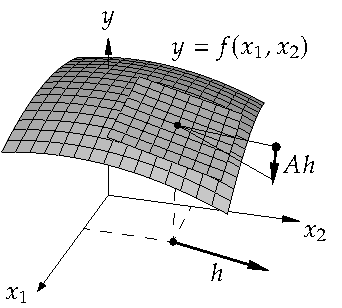
\includegraphics{figures/svder}
\caption{Illustration of a derivative for a function $f \colon \R^2 \to \R$.  The vector $h$ is shown
in the $x_1x_2$-plane based at $(x_1,x_2)$, and the vector
$Ah \in \R^1$ is shown along the $y$ direction.\label{fig:svder}}
\end{myfigureht}

For a differentiable function,
the derivative of $f$ is a function from $U$ to $L(\R^n,\R^m)$.  Compare
to the one-dimensional case, where the derivative is a function
from $U$ to $\R$, but we really want to think of $\R$ here as
$L(\R^1,\R^1)$.  As in one dimension, the idea is that a differentiable
mapping is \myquote{infinitesimally close} to a linear mapping, and this
linear mapping is the derivative.

Notice the norms in the definition.
The norm in the
numerator is on $\R^m$, and the norm in the denominator is on $\R^n$ where $h$
lives.
Normally it is understood that $h \in \R^n$ from context
(the formula makes no sense otherwise).
We will not explicitly say so from now on.
Let us prove, as promised, that the derivative is unique.

%We have again cheated somewhat and said that $A$
%is \emph{the} derivative.  We have not shown yet that there
%is only one, let us do that now.

\begin{prop}
Let $U \subset \R^n$ be an open subset and $f \colon U \to \R^m$ a function.  Suppose
$x \in U$ and there exist 
$A,B \in L(\R^n,\R^m)$ such that
\begin{equation*}
\lim_{h \to 0}
\frac{\snorm{f(x+h)-f(x) - Ah}}{\snorm{h}} = 0
\qquad \text{and} \qquad
\lim_{h \to 0}
\frac{\snorm{f(x+h)-f(x) - Bh}}{\snorm{h}} = 0 .
\end{equation*}
Then $A=B$.
\end{prop}

\begin{proof}
Suppose $h \in \R^n$, $h \not= 0$.  Compute
\begin{equation*}
\begin{split}
\frac{\snorm{(A-B)h}}{\snorm{h}} & =
\frac{\snorm{-\bigl(f(x+h)-f(x) - Ah\bigr) + f(x+h)-f(x) - Bh}}{\snorm{h}} \\
& \leq
\frac{\snorm{f(x+h)-f(x) - Ah}}{\snorm{h}} + \frac{\snorm{f(x+h)-f(x) -
Bh}}{\snorm{h}} .
\end{split}
\end{equation*}
So 
$\frac{\snorm{(A-B)h}}{\snorm{h}} \to 0$ as $h \to 0$.  Given
$\epsilon > 0$, for all nonzero $h$ in some $\delta$-ball around
the origin we have
\begin{equation*}
\epsilon > 
\frac{\snorm{(A-B)h}}{\snorm{h}}
=
\norm{(A-B)\frac{h}{\snorm{h}}} .
\end{equation*}
For any given $v \in \R^n$ with $\snorm{v}=1$,
if $h = (\nicefrac{\delta}{2}) \, v$, then $\snorm{h} < \delta$
and $\frac{h}{\snorm{h}} = v$.
So $\snorm{(A-B)v} < \epsilon$.  Taking the supremum over all $v$ with
$\snorm{v} = 1$, we get the operator norm
$\snorm{A-B} \leq \epsilon$.  As $\epsilon > 0$
was arbitrary, $\snorm{A-B} = 0$, or in other words $A = B$.
\end{proof}

\begin{example}
If $f(x) = Ax$ for a linear mapping $A$, then
$f'(x) = A$:
\begin{equation*}
\frac{\snorm{f(x+h)-f(x) - Ah}}{\snorm{h}}
=
\frac{\snorm{A(x+h)-Ax - Ah}}{\snorm{h}}
=
\frac{0}{\snorm{h}} = 0 .
\end{equation*}
\end{example}

\begin{example}
Let $f \colon \R^2 \to \R^2$ be defined by
\begin{equation*}
f(x,y) = \bigl(f_1(x,y),f_2(x,y)\bigr) \coloneqq (1+x+2y+x^2,2x+3y+xy).
\end{equation*}
Let us show that $f$ is differentiable at the origin and
compute the derivative directly using the definition.
If the derivative exists, it is in $L(\R^2,\R^2)$, so it can be
represented by a $2$-by-$2$ matrix
$\left[\begin{smallmatrix}a&b\\c&d\end{smallmatrix}\right]$.  Suppose $h =
(h_1,h_2)$.  We need the following expression to go to zero.
\begin{multline*}
\frac{\snorm{
f(h_1,h_2)-f(0,0)
-
(ah_1 +bh_2 , ch_1+dh_2)}
}{\snorm{(h_1,h_2)}}
=
\\
\frac{\sqrt{
{\bigl((1-a)h_1 + (2-b)h_2 + h_1^2\bigr)}^2
+
{\bigl((2-c)h_1 + (3-d)h_2 + h_1h_2\bigr)}^2}}{\sqrt{h_1^2+h_2^2}} .
\end{multline*}
If we choose $a=1$, $b=2$, $c=2$, $d=3$, the expression becomes
\begin{equation*}
\frac{\sqrt{
h_1^4 + h_1^2h_2^2}}{\sqrt{h_1^2+h_2^2}}
=
\sabs{h_1}
\frac{\sqrt{
h_1^2 + h_2^2}}{\sqrt{h_1^2+h_2^2}}
= \sabs{h_1} .
\end{equation*}
This expression does indeed go to zero as $h \to 0$.  The
function $f$ is differentiable at the origin and 
the derivative $f'(0)$ is represented by the matrix
$\left[\begin{smallmatrix}1&2\\2&3\end{smallmatrix}\right]$.
\end{example}

\begin{prop}
Let $U \subset \R^n$ be open and $f \colon U \to \R^m$ be
differentiable at $p \in U$.  Then $f$ is continuous at $p$.
\end{prop}

\begin{proof}
Another way to write the differentiability of $f$ at $p$ is to consider
\begin{equation*}
r(h) \coloneqq f(p+h)-f(p) - f'(p) h .
\end{equation*}
The function $f$ is differentiable at $p$ if
$\frac{\snorm{r(h)}}{\snorm{h}}$ goes to zero as $h \to 0$,
so
$r(h)$ itself goes to zero.  The mapping $h \mapsto f'(p) h$
is a linear mapping between finite-dimensional spaces, hence continuous
and $f'(p) h \to 0$ as $h \to 0$.  Thus,
$f(p+h)$ must go to $f(p)$ as $h \to 0$.  That is, $f$ is continuous at $p$.
\end{proof}

Differentiation is a linear operator on the space of differentiable
functions.

\begin{prop}
Suppose $U \subset \R^n$ is open,
$f \colon U \to \R^m$ and
$g \colon U \to \R^m$ are differentiable at $p \in U$,
and $\alpha \in \R$.  Then the functions $f+g$ and $\alpha f$
are differentiable at $p$,
\begin{equation*}
(f+g)'(p) = f'(p) + g'(p) , \qquad \text{and} \qquad (\alpha f)'(p) = \alpha
f'(p) .
\end{equation*}
\end{prop}

\begin{proof}
Let $h \in \R^n$, $h \not= 0$.  Then
\begin{multline*}
\frac{\norm{f(p+h)+g(p+h)-\bigl(f(p)+g(p)\bigr) - \bigl(f'(p) + g'(p)\bigr)h}}{\snorm{h}}
\\
\leq
\frac{\norm{f(p+h)-f(p) - f'(p)h}}{\snorm{h}}
+
\frac{\norm{g(p+h)-g(p) - g'(p)h}}{\snorm{h}} ,
\end{multline*}
and
\begin{equation*}
\frac{\norm{\alpha f(p+h) - \alpha f(p) - \alpha f'(p)h}}{\snorm{h}}
=
\sabs{\alpha} \frac{\norm{f(p+h))-f(p) - f'(p)h}}{\snorm{h}} .
\end{equation*}
The limits as $h$ goes to zero of the right-hand sides are zero by
hypothesis.  The result follows.
\end{proof}

If $A \in L(\R^n,\R^m)$ and $B \in L(\R^m,\R^k)$ are linear maps, then 
they are their own derivative.  The composition
$BA \in L(\R^n,\R^k)$ is also its own derivative, and
so the derivative of the composition is the composition
of the derivatives.  As differentiable maps are
\myquote{infinitesimally close}
to linear maps, they have the same property:

\begin{thm}[Chain rule] \index{chain rule}
Let $U \subset \R^n$ and $V \subset \R^m$ be open sets, $f \colon U \to
\R^m$ be differentiable at $p \in U$, $f(U) \subset V$,
and let $g \colon V \to \R^\ell$ be differentiable
at $f(p)$.  Then $F \colon U \to \R^{\ell}$ defined by
\begin{equation*}
F(x) \coloneqq g\bigl(f(x)\bigr)
\end{equation*}
is differentiable at $p$, and
\begin{equation*}
F'(p) = g'\bigl(f(p)\bigr) f'(p) .
\end{equation*}
\end{thm}

Without the points where things are evaluated, we write
$F' = {(g \circ f)}' = g' f'$.
The derivative of the composition $g \circ f$
is the composition of the derivatives of $g$ and $f$:
If $f'(p) = A$ and $g'\bigl(f(p)\bigr) = B$, then $F'(p) = BA$,
just as for linear maps.

\begin{proof}
Let $A \coloneqq f'(p)$ and $B \coloneqq g'\bigl(f(p)\bigr)$.  Take a nonzero $h \in \R^n$
and write $q \coloneqq f(p)$, $k \coloneqq f(p+h)-f(p)$.  Let
\begin{equation*}
r(h) \coloneqq f(p+h)-f(p) - A h . %= k - Ah.
\end{equation*}
Then $r(h) = k-Ah$ or $Ah = k-r(h)$, and $f(p+h) = q+k$.
We look at the quantity we need to go
to zero:
\begin{equation*}
\begin{split}
\frac{\snorm{F(p+h)-F(p) - BAh}}{\snorm{h}}
& =
\frac{\snorm{g\bigl(f(p+h)\bigr)-g\bigl(f(p)\bigr) - BAh}}{\snorm{h}}
\\
& =
\frac{\snorm{g(q+k)-g(q) - B\bigl(k-r(h)\bigr)}}{\snorm{h}}
\\
& \leq
\frac
{\snorm{g(q+k)-g(q) - Bk}}
{\snorm{h}}
+
\snorm{B}
\frac
{\snorm{r(h)}}
{\snorm{h}}
\\
& =
\frac
{\snorm{g(q+k)-g(q) - Bk}}
{\snorm{k}}
\frac
{\snorm{f(p+h)-f(p)}}
{\snorm{h}}
+
\snorm{B}
\frac
{\snorm{r(h)}}
{\snorm{h}} .
\end{split}
\end{equation*}
First, $\snorm{B}$ is a constant and $f$ is differentiable at $p$,
so
the term $\snorm{B}\frac{\snorm{r(h)}}{\snorm{h}}$ goes to 0.
Next, because $f$ is continuous at $p$,
$k$ goes to 0 as $h$ goes to 0.
Thus
$\frac
{\snorm{g(q+k)-g(q) - Bk}}
{\snorm{k}}$ goes to 0, because $g$ is differentiable at $q$.
Finally,
\begin{equation*}
\frac
{\snorm{f(p+h)-f(p)}}
{\snorm{h}}
\leq
\frac
{\snorm{f(p+h)-f(p)-Ah}}
{\snorm{h}}
+
\frac
{\snorm{Ah}}
{\snorm{h}}
\leq
\frac
{\snorm{f(p+h)-f(p)-Ah}}
{\snorm{h}}
+
\snorm{A} .
\end{equation*}
As $f$ is differentiable at $p$,
for small enough $h$, the quantity
$\frac{\snorm{f(p+h)-f(p)-Ah}}{\snorm{h}}$ is bounded.  Hence, the
term
$
\frac
{\snorm{f(p+h)-f(p)}}
{\snorm{h}}
$
stays bounded as $h$ goes to 0.  Therefore, 
$\frac{\snorm{F(p+h)-F(p) - BAh}}{\snorm{h}}$ goes to zero, and
$F'(p) = BA$, which is what was claimed.
\end{proof}

\subsection{Partial derivatives}

There is another way to generalize the derivative from one dimension.
We hold all but one variable constant and take the regular
one-variable derivative.

\begin{defn}
Let
$f \colon U \to \R$ be a function on an open set $U \subset \R^n$.
If the following limit exists, we write
\glsadd{not:partialder}
\begin{equation*}
\frac{\partial f}{\partial x_j} (x) \coloneqq 
\lim_{h\to 0}\frac{f(x_1,\ldots,x_{j-1},x_j+h,x_{j+1},\ldots,x_n)-f(x)}{h}
=
\lim_{h\to 0}\frac{f(x+h e_j)-f(x)}{h} .
\end{equation*}
We call 
$\frac{\partial f}{\partial x_j} (x)$ the \emph{\myindex{partial derivative}}
of $f$
with respect to $x_j$.  %Sometimes we write $D_j f$ instead.
See \figureref{fig:svpartder}.
Here $h$ is a number, not a vector.

For a mapping $f \colon U \to \R^m$, we write
$f = (f_1,f_2,\ldots,f_m)$, where $f_k$ are real-valued
functions.  We then take partial derivatives of
the components,
$\frac{\partial f_k}{\partial x_j}$.
\end{defn}

\begin{myfigureht}
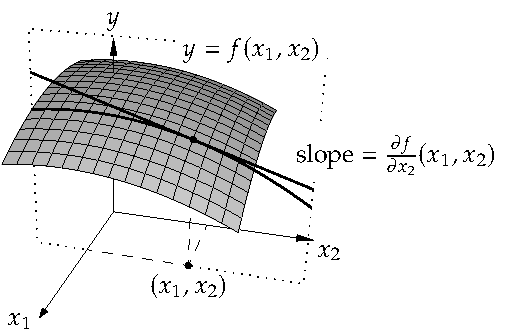
\includegraphics{figures/svpartder}
\caption{Illustration of a partial derivative for a function $f \colon \R^2
\to \R$.  The $yx_2$-plane where $x_1$ is fixed is marked in dotted line,
and the slope of the tangent line in the $yx_2$-plane is
$\frac{\partial f}{\partial x_2}(x_1,x_2)$.\label{fig:svpartder}}
\end{myfigureht}

Partial derivatives are easier to compute with all the machinery of
calculus, and they provide a way to compute the derivative of a
function.

\begin{prop} \label{mv:prop:jacobianmatrix}
Let $U \subset \R^n$ be open and let $f \colon U \to \R^m$ be
differentiable at $p \in U$.  Then all the partial derivatives at $p$
exist and, in terms of the standard bases of $\R^n$ and $\R^m$,
$f'(p)$ is represented by the matrix
\begin{equation*}
\begin{bmatrix}
\frac{\partial f_1}{\partial x_1}(p)
&
\frac{\partial f_1}{\partial x_2}(p)
& \ldots &
\frac{\partial f_1}{\partial x_n}(p)
\\[6pt]
\frac{\partial f_2}{\partial x_1}(p)
&
\frac{\partial f_2}{\partial x_2}(p)
& \ldots &
\frac{\partial f_2}{\partial x_n}(p)
\\
\vdots & \vdots & \ddots & \vdots
\\
\frac{\partial f_m}{\partial x_1}(p)
&
\frac{\partial f_m}{\partial x_2}(p)
& \ldots &
\frac{\partial f_m}{\partial x_n}(p)
\end{bmatrix} .
\end{equation*}
\end{prop}


In other words,
\begin{equation*}
f'(p) \, e_j =
\sum_{k=1}^m
\frac{\partial f_k}{\partial x_j}(p) \,e_k .
\end{equation*}
If $v = \sum_{j=1}^n c_j\, e_j = (c_1,c_2,\ldots,c_n)$, then
\begin{equation*}
f'(p) \, v =
\sum_{j=1}^n
\sum_{k=1}^m
 c_j
\frac{\partial f_k}{\partial x_j}(p) \,e_k
=
\sum_{k=1}^m
\left(
\sum_{j=1}^n
 c_j
\frac{\partial f_k}{\partial x_j}(p) \right) \,e_k .
\end{equation*}

\begin{proof}
Fix a $j$ and note that for nonzero $h$,
\begin{equation*}
\begin{split}
\norm{\frac{f(p+h e_j)-f(p)}{h} - f'(p) \, e_j} & = 
\norm{\frac{f(p+h e_j)-f(p) - f'(p) \, h e_j}{h}} \\
& =
\frac{\snorm{f(p+h e_j)-f(p) - f'(p) \, h e_j}}{\snorm{h e_j}} .
\end{split}
\end{equation*}
As $h$ goes to 0, the right-hand side goes to zero by
differentiability of $f$.  Hence,
\begin{equation*}
\lim_{h \to 0}
\frac{f(p+h e_j)-f(p)}{h} = f'(p) \, e_j  .
\end{equation*}
The limit is in $\R^m$.
Represent $f$ in components
$f = (f_1,f_2,\ldots,f_m)$.
Taking a limit in $\R^m$
is the same as taking the limit in each component separately.  
So for every $k$,
the partial derivative
\begin{equation*}
\frac{\partial f_k}{\partial x_j} (p)
=
\lim_{h \to 0}
\frac{f_k(p+h e_j)-f_k(p)}{h}
\end{equation*}
exists and is equal to the $k$th component of $f'(p)\, e_j$, which is the
$j$th column of $f'(p)$,
and we are done.
\end{proof}

The converse of the proposition is not true.  Just because the partial
derivatives exist, does not mean that the function is differentiable.  See
the exercises.
However, when the partial derivatives are continuous, we will prove that the
converse holds.
One of the consequences of the proposition above is that if $f$
is differentiable on $U$, then $f' \colon U \to
L(\R^n,\R^m)$ is a continuous function if and only if
all the $\frac{\partial f_k}{\partial x_j}$ are continuous functions.

\subsection{Gradients, curves, and directional derivatives}

Let $U \subset \R^n$ be open and $f \colon U \to \R$ a differentiable
function.  We define
the \emph{\myindex{gradient}} as
\glsadd{not:gradient}
\begin{equation*}
\nabla f (x) \coloneqq \sum_{j=1}^n \frac{\partial f}{\partial x_j} (x)\, e_j .
\end{equation*}
The gradient gives a way to represent the action of
the derivative as a dot product: $f'(x)\,v = \nabla f(x) \cdot v$.

Suppose $\gamma \colon (a,b) \subset \R \to \R^n$ is differentiable.
Such a function and its image is sometimes called a \emph{\myindex{curve}},
or a \emph{\myindex{differentiable curve}}.
Write $\gamma =
(\gamma_1,\gamma_2,\ldots,\gamma_n)$.
For the purposes of computation,
we identify $L(\R^1)$ and $\R$ as we did when we defined the
derivative in one variable.
We also identify $L(\R^1,\R^n)$ with $\R^n$.
We treat $\gamma^{\:\prime}(t)$ both as an operator in
$L(\R^1,\R^n)$ and the vector
$\bigl(\gamma_1^{\:\prime}(t),
\gamma_2^{\:\prime}(t),\ldots,\gamma_n^{\:\prime}(t)\bigr)$
in $\R^n$.
Using \propref{mv:prop:jacobianmatrix},
if $v\in \R^n$ is $\gamma^{\:\prime}(t)$ acting as a vector,
then $h \mapsto h \, v$ (for $h \in \R^1 = \R$) is
$\gamma^{\:\prime}(t)$ acting as an operator
in $L(\R^1,\R^n)$.
We often use this 
slight abuse of notation when dealing with curves.
The vector $\gamma^{\:\prime}(t)$ is called a \emph{\myindex{tangent vector}}.
See \figureref{fig:difcurveder}.
\begin{myfigureht}
\subimport*{figures/}{diffcurveder.pdf_t}
\caption{Differentiable curve and its derivative as a
vector (for clarity assuming $\gamma$ defined on $[a,b]$).
The tangent vector $\gamma^{\:\prime}(t)$ points along the curve.\label{fig:difcurveder}}
\end{myfigureht}

Suppose $\gamma\bigl((a,b)\bigr) \subset U$ and let
\begin{equation*}
g(t) \coloneqq f\bigl(\gamma(t)\bigr) .
\end{equation*}
The function
$g$ is differentiable. Treating $g'(t)$ as a number,
\begin{equation*}
g'(t) =
f'\bigl(\gamma(t)\bigr) \gamma^{\:\prime}(t)
=
\sum_{j=1}^n
\frac{\partial f}{\partial x_j} \bigl(\gamma(t)\bigr)
\frac{d\gamma_j}{dt} (t)
=
\sum_{j=1}^n
\frac{\partial f}{\partial x_j}
\frac{d\gamma_j}{dt} .
\end{equation*}
For convenience,
we often 
leave out the points where we are evaluating,
such as above on the far right-hand side.
With the notation of the gradient and the dot product
the equation becomes
\begin{equation*}
g'(t) = (\nabla f) \bigl(\gamma(t)\bigr) \cdot \gamma^{\:\prime}(t)
= \nabla f \cdot \gamma^{\:\prime}.
\end{equation*}

We use this idea to define derivatives in a specific direction.  A direction
is simply a vector pointing in that direction.  Pick a vector $u \in \R^n$
such that $\snorm{u} = 1$, and fix $x \in U$.
We define the
\emph{\myindex{directional derivative}} as
\glsadd{not:mvdirder}
\begin{equation*}
D_u f (x) \coloneqq \frac{d}{dt}\Big|_{t=0} \bigl[ f(x+tu) \bigr] =
\lim_{h\to 0}
\frac{f(x+hu)-f(x)}{h} ,
\end{equation*}
where the notation
$\frac{d}{dt}\big|_{t=0}$ represents the derivative evaluated at $t=0$.
When $u=e_j$ is a standard basis vector, we find
$\frac{\partial f}{\partial x_j} = D_{e_j} f$.
For this reason, sometimes the notation $\frac{\partial f}{\partial u}$
is used instead of $D_u f$.

Define $\gamma$ by
\begin{equation*}
\gamma(t) \coloneqq x + tu .
\end{equation*}
Then $\gamma^{\:\prime}(t) = u$ for all $t$.  
Let us see what happens to $f$ when we travel along $\gamma$:
\begin{equation*}
D_u f (x) =
\frac{d}{dt}\Big|_{t=0} \bigl[ f(x+tu) \bigr] =
(\nabla f) \bigl(\gamma(0)\bigr) \cdot \gamma^{\:\prime}(0)
=
(\nabla f) (x) \cdot u .
\end{equation*}
In fact, this computation holds whenever $\gamma$ is any curve such that
$\gamma(0) = x$ and $\gamma^{\:\prime}(0) = u$.

Suppose $(\nabla f)(x) \neq 0$.
By the Cauchy--Schwarz inequality,
\begin{equation*}
\sabs{D_u f(x)} \leq \snorm{(\nabla f)(x)} .
\end{equation*}
Equality is achieved when $u$ is a scalar multiple of
$(\nabla f)(x)$.  That is, when
\begin{equation*}
u = 
\frac{(\nabla f)(x)}{\snorm{(\nabla f)(x)}} ,
\end{equation*}
we get $D_u f(x) = \snorm{(\nabla f)(x)}$.
The gradient points in the direction in which the
function grows fastest, in other words,
in the direction in which $D_u f(x)$ is maximal.

\subsection{The Jacobian}

\begin{defn}
Let $U \subset \R^n$ and
$f \colon U \to \R^n$ be a differentiable mapping.  Define the
\emph{\myindex{Jacobian determinant}}%
\footnote{Named after the Italian mathematician
\href{https://en.wikipedia.org/wiki/Carl_Gustav_Jacob_Jacobi}{Carl Gustav Jacob Jacobi}
(1804--1851).},
or simply the
\emph{\myindex{Jacobian}}%
\footnote{The matrix from \propref{mv:prop:jacobianmatrix} representing $f'(x)$
is called the
\emph{\myindex{Jacobian matrix}}, or sometimes confusingly also called just ``the
Jacobian.''},
of $f$ at $x$ as
\glsadd{not:jacobdet}
\begin{equation*}
J_f(x) \coloneqq \det\bigl( f'(x) \bigr) .
\end{equation*}
Sometimes $J_f$ is written as
\begin{equation*}
\frac{\partial(f_1,f_2,\ldots,f_n)}{\partial(x_1,x_2,\ldots,x_n)} .
\end{equation*}
\end{defn}

This last piece of notation may seem somewhat confusing,
but it is quite useful when we need to specify
the exact variables and function components used,
as we will do, for example, in the implicit function theorem.

The Jacobian determinant $J_f$ is a real-valued function, and when $n=1$ it is simply the
derivative.
From the chain rule and the fact that $\det(AB) = \det(A)\det(B)$, it follows that:
\begin{equation*}
J_{f \circ g} (x) = J_f\bigl(g(x)\bigr) J_g(x) .
\end{equation*}

The determinant of a linear mapping tells us what happens to
area/volume under the mapping.
Similarly, the Jacobian determinant measures how much a differentiable mapping stretches
things locally, and if it flips orientation.  In particular, if the Jacobian
determinant
is non-zero than we would assume that locally the mapping is invertible (and
we would be correct as we will later see).

\subsection{Exercises}

\begin{exercise}
Suppose $\gamma \colon (-1,1) \to \R^n$ and
$\alpha \colon (-1,1) \to \R^n$ are two differentiable curves
such that $\gamma(0) = \alpha(0)$ and $\gamma^{\:\prime}(0) = \alpha'(0)$.
Suppose $F \colon \R^n \to \R$ is a differentiable function.  Show that
\begin{equation*}
\frac{d}{dt}\Big|_{t=0}
F\bigl(\gamma(t)\bigr)
=
\frac{d}{dt}\Big|_{t=0}
F\bigl(\alpha(t)\bigr)
.
\end{equation*}
\end{exercise}

\begin{exercise}
Let $f \colon \R^2 \to \R$ be given by
$f(x,y)
\coloneqq
\sqrt{x^2+y^2}$,
see \figureref{fig:distfromorgfunc}.
Show that $f$ is not differentiable at the origin.
\end{exercise}

\begin{myfigureht}
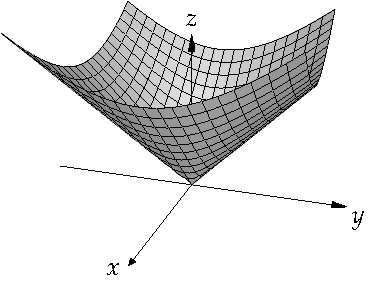
\includegraphics{figures/distfromorgfunc}
\caption{Graph of $\sqrt{x^2+y^2}$.\label{fig:distfromorgfunc}}
\end{myfigureht}

\begin{samepage}
\begin{exercise}
Using only the definition of the derivative, show that
the following $f \colon \R^2 \to \R^2$ are differentiable at the origin and
find their derivative.
\begin{enumerate}[a)]
\item
$f(x,y) \coloneqq (1+x+xy,x)$,
\item
$f(x,y) \coloneqq \bigl(y-y^{10},x \bigr)$,
\item
$f(x,y) \coloneqq \bigl( {(x+y+1)}^2 , {(x-y+2)}^2 \bigr)$.
\end{enumerate}
\end{exercise}
\end{samepage}

\begin{exercise}
Suppose $f \colon \R \to \R$ and $g \colon \R \to \R$ are differentiable
functions.  Using only the definition of the derivative, show that
$h \colon \R^2 \to \R^2$ defined by $h(x,y)
\coloneqq \bigl(f(x),g(y)\bigr)$ is a differentiable function, and find the
derivative, at all points $(x,y)$.
\end{exercise}

\begin{exercise} \label{exercise:noncontpartialsexist}
Define a function $f \colon \R^2 \to \R$ by
(see \figureref{fig:xyxsqysqvol2})
\begin{equation*}
f(x,y)
\coloneqq
\begin{cases}
\frac{xy}{x^2+y^2} & \text{if } (x,y) \not= (0,0), \\
0                  & \text{if } (x,y) = (0,0).
\end{cases}
\end{equation*}
\begin{enumerate}[a)]
\item
Show that the partial derivatives 
$\frac{\partial f}{\partial x}$ and
$\frac{\partial f}{\partial y}$ exist at all points (including the origin).
\item
Show that $f$ is not continuous at the origin (and hence not
differentiable).
\end{enumerate}
\end{exercise}

\begin{myfigureht}
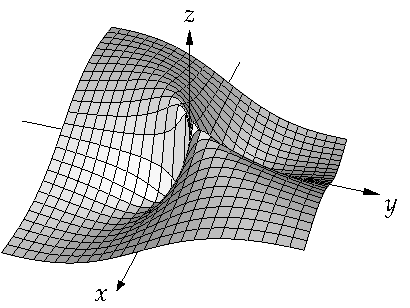
\includegraphics{figures/xyxsqysq}
\caption{Graph of $\frac{xy}{x^2+y^2}$.\label{fig:xyxsqysqvol2}}
\end{myfigureht}

\begin{samepage}
\begin{exercise}
Define a function $f \colon \R^2 \to \R$ by
(see \figureref{fig:xsqyxsqysq})
\begin{equation*}
f(x,y)
\coloneqq
\begin{cases}
\frac{x^2y}{x^2+y^2} & \text{if } (x,y) \not= (0,0), \\
0                    & \text{if } (x,y) = (0,0).
\end{cases}
\end{equation*}
\begin{enumerate}[a)]
\item
Show that the partial derivatives 
$\frac{\partial f}{\partial x}$ and
$\frac{\partial f}{\partial y}$ exist at all points.
\item
Show that for all $u \in \R^2$ with $\snorm{u}=1$, the directional
derivative $D_u f$ exists at all points.
\item
Show that $f$ is continuous at the origin.
\item
Show that $f$ is not differentiable at the origin.
\end{enumerate}
\end{exercise}
\end{samepage}

\begin{myfigureht}
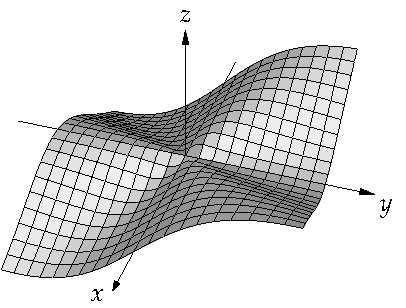
\includegraphics{figures/xsqyxsqysq}
\caption{Graph of $\frac{x^2y}{x^2+y^2}$.\label{fig:xsqyxsqysq}}
\end{myfigureht}

\begin{samepage}
\begin{exercise}
Suppose $f \colon \R^n \to \R^n$ is one-to-one, onto, differentiable at all
points, and such that $f^{-1}$ is also differentiable at all points.
\begin{enumerate}[a)]
\item
Show that $f'(p)$ is invertible at all points $p$ and compute
${(f^{-1})}'\bigl(f(p)\bigr)$.  Hint: Consider $x = f^{-1}\bigl(f(x)\bigr)$.
\item
Let $g \colon \R^n \to \R^n$ be a function differentiable at $q \in \R^n$
and such that $g(q)=q$.  Suppose $f(p) = q$ for some $p \in \R^n$.
Show $J_g(q) = J_{f^{-1} \circ g \circ f}(p)$ where $J_g$ is the Jacobian
determinant.
\end{enumerate}
\end{exercise}
\end{samepage}

\begin{exercise}
Suppose $f \colon \R^2 \to \R$ is differentiable and such that
$f(x,y) = 0$ if and only if $y=0$ and such that $\nabla f(0,0) = (0,1)$.
Prove that $f(x,y) > 0$ whenever $y > 0$, and
$f(x,y) < 0$ whenever $y < 0$.
\end{exercise}

\begin{exnote}
\pagebreak[2]
As for functions of one variable, $f \colon U \to \R$ has a
\emph{\myindex{relative maximum}} at $p \in U$ if there exists
a $\delta >0$ such that $f(q) \leq f(p)$ for all $q \in B(p,\delta) \cap U$.
Similarly for \emph{\myindex{relative minimum}}.
\end{exnote}

\begin{exercise} \label{exercise:mv:maximumcritical}
Suppose $U \subset \R^n$ is open and
$f \colon U \to \R$ is differentiable.  Suppose $f$ has a relative maximum
at $p \in U$.  Show that $f'(p) = 0$, that is, the zero mapping in
$L(\R^n,\R)$.  Namely, $p$ is a
\emph{\myindex{critical point}} of $f$.
\end{exercise}

\begin{exercise}
Suppose $f \colon \R^2 \to \R$ is differentiable and 
$f(x,y) = 0$ whenever $x^2+y^2 = 1$.
Prove that there exists at least
one point $(x_0,y_0)$ such that
$\frac{\partial f}{\partial x}(x_0,y_0) = \frac{\partial f}{\partial
y}(x_0,y_0) = 0$.
\end{exercise}

\begin{exercise} \label{exercise:peano}
Define $f(x,y) \coloneqq ( x-y^2 ) ( 2 y^2 - x)$.  The graph of $f$ is called
the \emph{\myindex{Peano surface}}.%
\footnote{Named after the Italian mathematician
\href{https://en.wikipedia.org/wiki/Giuseppe_Peano}{Giuseppe Peano}
(1858--1932).}
\begin{enumerate}[a)]
\item
Show that
$(0,0)$ is a critical point, that is $f'(0,0) = 0$, that is the zero
linear map in $L(\R^2,\R)$.
\item
Show that for every direction the restriction of $f$ to a line through the origin
in that direction has a relative maximum at the origin.  In other words,
for every $(x,y)$ such that $x^2+y^2=1$, the function $g(t) \coloneqq f(tx,ty)$,
has a relative maximum at $t=0$.\\
Hint: While not necessary
\volIref{\sectionref*{vI-sec:taylor} of volume I}{\sectionref{sec:taylor}}
makes
this part easier.
\item
Show that $f$ does not have a relative maximum at $(0,0)$.
\end{enumerate}
\end{exercise}

\begin{exercise}
Suppose $f \colon \R \to \R^n$ is differentiable and $\snorm{f(t)} = 1$ for
all $t$ (that is, we have a curve in the unit sphere).  Show that 
$f'(t) \cdot f(t) = 0$ (treating $f'(t)$ as a vector) for all $t$.
\end{exercise}

\begin{exercise}
Define $f \colon \R^2 \to \R^2$ by $f(x,y) \coloneqq
\bigl(x,y+\varphi(x)\bigr)$ for some differentiable function $\varphi$ of one
variable.  Show $f$ is differentiable and find $f'$.
\end{exercise}

\begin{exercise}
Suppose $U \subset \R^n$ is open, $p \in U$, and
$f \colon U \to \R$,
$g \colon U \to \R$,
$h \colon U \to \R$ are functions such that
$f(p) = g(p) = h(p)$, $f$ and $h$ are differentiable at $p$,
$f'(p) = h'(p)$, and
\begin{equation*}
f(x) \leq g(x) \leq h(x) \qquad \text{for all } x \in U
\end{equation*}
Show that $g$ is differentiable at $p$ and 
$g'(p) = f'(p) = h'(p)$.
\end{exercise}

\begin{exercise}
Prove a version of \emph{\myindex{mean value theorem}}
for functions of several variables.  That is, suppose $U \subset \R^n$
is open, $f \colon U \to \R$ differentiable, $p,q \in U$, and the segment
$[p,q] \in U$.  Prove that there exists an $x \in [p,q]$ such that
$\nabla f (x) \cdot (q-p) = f(q)-f(p)$.
\end{exercise}

%%%%%%%%%%%%%%%%%%%%%%%%%%%%%%%%%%%%%%%%%%%%%%%%%%%%%%%%%%%%%%%%%%%%%%%%%%%%%%

\sectionnewpage
\section{Continuity and the derivative}
\label{sec:svthedercont}

\sectionnotes{1--2 lectures}

\subsection{Bounding the derivative}

Let us prove a \myquote{\myindex{mean value theorem}} for vector-valued functions.

\begin{lemma} \label{lemma:mvtmv}
If $\varphi \colon [a,b] \to \R^n$ is differentiable on $(a,b)$ and
continuous on $[a,b]$, then there exists a $t_0 \in (a,b)$ such that
\begin{equation*}
\snorm{\varphi(b)-\varphi(a)} \leq (b-a) \snorm{\varphi'(t_0)} .
\end{equation*}
\end{lemma}

\begin{proof}
By the mean value theorem on the scalar-valued function
$t \mapsto \bigl(\varphi(b)-\varphi(a) \bigr) \cdot \varphi(t)$,
where the dot is the dot product, we obtain
a $t_0 \in (a,b)$ such that
\begin{equation*}
\begin{split}
\snorm{\varphi(b)-\varphi(a)}^2
& =
\bigl( \varphi(b)-\varphi(a) \bigr)
\cdot
\bigl( \varphi(b)-\varphi(a) \bigr)
\\
& =
\bigl(\varphi(b)-\varphi(a) \bigr) \cdot \varphi(b) - 
\bigl(\varphi(b)-\varphi(a) \bigr) \cdot \varphi(a)
\\
& = 
(b-a)
\bigl(\varphi(b)-\varphi(a) \bigr) \cdot \varphi'(t_0) ,
\end{split}
\end{equation*}
where we treat $\varphi'$ as a vector in $\R^n$ by the abuse of
notation we mentioned in the previous section.
If we think of $\varphi'(t)$ as a vector, then by
\exerciseref{exercise:normonedim},
$\snorm{\varphi'(t)}_{L(\R,\R^n)} = \snorm{\varphi'(t)}_{\R^n}$.
That is, the euclidean norm of the vector is the same as the operator norm
of $\varphi'(t)$.

By the Cauchy--Schwarz inequality
\begin{equation*}
\snorm{\varphi(b)-\varphi(a)}^2
=
(b-a)\bigl(\varphi(b)-\varphi(a) \bigr) \cdot \varphi'(t_0)
\leq
(b-a)
\snorm{\varphi(b)-\varphi(a)} \, \snorm{\varphi'(t_0)} . \qedhere
\end{equation*}
\end{proof}

Recall that a set $U$ is convex
if whenever $p,q \in U$, the line segment from
$p$ to $q$ lies in $U$.

\begin{prop} \label{mv:prop:convexlip}
Let $U \subset \R^n$ be a convex open set, $f \colon U \to \R^m$
be a differentiable function, and an $M$ be such that
\begin{equation*}
\snorm{f'(p)} \leq M
\qquad \text{for all } p \in U.
\end{equation*}
Then $f$ is Lipschitz with constant $M$, that is,
\begin{equation*}
\snorm{f(p)-f(q)} \leq M \snorm{p-q}
\qquad
\text{for all } p,q \in U.
\end{equation*}
\end{prop}

\begin{proof}
Fix $p$ and $q$ in $U$ and note that
$(1-t)p+tq \in U$ for all $t \in [0,1]$
by convexity.
Next
\begin{equation*}
\frac{d}{dt} \Bigl[f\bigl((1-t)p+tq\bigr)\Bigr]
=
f'\bigl((1-t)p+tq\bigr) (q-p) .
\end{equation*}
By \lemmaref{lemma:mvtmv}, there is some
$t_0 \in (0,1)$ such that
\begin{equation*}
\begin{split}
\snorm{f(p)-f(q)} & \leq
\norm{\frac{d}{dt} \Big|_{t=t_0} \Bigl[ f\bigl((1-t)p+tq\bigr) \Bigr] }
\\
& \leq
\norm{f'\bigl((1-t_0)p+t_0q\bigr)} \, \snorm{q-p} \leq
M \snorm{q-p} . \qedhere
\end{split}
\end{equation*}
\end{proof}

\begin{example}
If $U$ is not convex the proposition is not true: Consider
the set
\begin{equation*}
U \coloneqq \bigl\{ (x,y) : 0.5 < x^2+y^2 < 2 \bigr\}
\setminus \bigl\{ (x,0) : x < 0 \bigr\} .
\end{equation*}
For $(x,y) \in U$,
let $f(x,y)$ be the angle that the line from the origin to $(x,y)$
makes with the positive $x$ axis.  We even have a formula for $f$:
\begin{equation*}
f(x,y) = 2 \operatorname{arctan}\left( \frac{y}{x+\sqrt{x^2+y^2}}\right) .
\end{equation*}
Think a spiral staircase with room in the middle.  See
\figureref{mv:fignonlip}.

\begin{myfigureht}
\subimport*{figures/}{nonlip_full.pdf_t}
\caption{A non-Lipschitz function with uniformly bounded
derivative.\label{mv:fignonlip}}
\end{myfigureht}

The function is differentiable,
and the derivative is bounded on $U$, which is not hard to see.   Now
think of
what happens near where the negative $x$-axis cuts the annulus in half.
As we approach this cut from positive $y$, $f(x,y)$ approaches $\pi$.
From negative $y$, $f(x,y)$ approaches $-\pi$.
So for small $\epsilon > 0$, $\sabs{f(-1,\epsilon)-f(-1,-\epsilon)}$
approaches $2\pi$, but $\snorm{(-1,\epsilon)-(-1,-\epsilon)} = 2\epsilon$,
which is arbitrarily small.  The conclusion of the proposition does not
hold for this nonconvex $U$.
\end{example}

Let us solve the differential equation $f' = 0$.

\begin{cor}
If $U \subset \R^n$ is open and connected, $f \colon U \to \R^m$ is
differentiable,
and $f'(x) = 0$ for all $x \in U$, then $f$ is constant.
\end{cor}

\begin{proof}
For any given $x \in U$, there is a ball $B(x,\delta) \subset U$.  The ball
$B(x,\delta)$ is convex.  Since
$\snorm{f'(y)} \leq 0$ for all $y \in B(x,\delta)$, then by the proposition,
$\snorm{f(x)-f(y)} \leq 0 \snorm{x-y} = 0$.  So $f(x) = f(y)$ for all $y \in
B(x,\delta)$.
Therefore, $f^{-1}(c)$ is open for all $c \in \R^m$.

Suppose $c_0 \in \R^m$ is such that
$f^{-1}(c_0) \not= \emptyset$. 
As $f$ is also continuous,
the two sets
\begin{equation*}
U' = f^{-1}(c_0), \qquad U'' = f^{-1}\bigl(\R^m\setminus\{c_0\}\bigr)
\end{equation*}
are open and disjoint, and further $U = U' \cup U''$.  As $U'$ is nonempty
and $U$ is connected, then
$U'' = \emptyset$.  So $f(x) = c_0$ for all $x \in U$.
\end{proof}

\subsection{Continuously differentiable functions}

\begin{defn}
Let $U \subset \R^n$ be open.
We say $f \colon U \to \R^m$ is
\emph{\myindex{continuously differentiable}},
or $C^1(U)$\glsadd{not:C1},
if $f$ is differentiable and $f' \colon U \to L(\R^n,\R^m)$
is continuous.
\end{defn}

\begin{prop} \label{mv:prop:contdiffpartials}
Let $U \subset \R^n$ be open and
$f \colon U \to \R^m$.  The function
$f$ is continuously differentiable if and only if 
the partial derivatives $\frac{\partial f_k}{\partial x_j}$
exist for all $k$ and $j$ and are continuous.
\end{prop}

Without continuity the theorem does not hold.  Just because
partial derivatives exist does not mean that $f$ is differentiable,
in fact, $f$ may not even be continuous.  See the exercises
for the last section and also for this section.

\begin{proof}
We proved that if $f$ is differentiable, then
the partial derivatives exist.  The partial
derivatives are the entries of the matrix representing $f'(x)$.  If
$f' \colon U \to L(\R^n,\R^m)$ is continuous, then the entries are
continuous, and hence the partial derivatives are continuous.

To prove the opposite direction,
suppose the partial derivatives exist and are continuous.
Fix $x \in U$.  If we show that $f'(x)$ exists we are done, because
the entries of the matrix representing $f'(x)$ are the partial
derivatives and if the entries are continuous functions,
the matrix-valued function $f'$ is continuous.

We do induction on dimension.  First,
the conclusion is true when $n=1$
(exercise, note that $f$ is vector-valued).
In this case, $f'(x)$ is essentially the derivative of
\volIref{\chapterref*{vI-der:chapter}}{\chapterref{der:chapter}}.
Suppose the conclusion is true for $\R^{n-1}$.
That is,
if we restrict to the first $n-1$ variables, the function is differentiable.
When taking the partial derivatives in $x_1$ through $x_{n-1}$,
it does not matter if we consider $f$ or $f$ restricted to the set where
$x_n$ is fixed.
In the following, by a slight abuse of notation,
we think of $\R^{n-1}$ as a subset of $\R^n$, that is, the set in $\R^n$ where $x_n = 0$.
In other words, we identify the vectors $(x_1,x_2,\ldots,x_{n-1})$ and
$(x_1,x_2,\ldots,x_{n-1},0)$.

Fix $p \in U$ and let
\begin{equation*}
A \coloneqq 
\begin{bmatrix}
\frac{\partial f_1}{\partial x_1}(p)
& \ldots &
\frac{\partial f_1}{\partial x_n}(p)
\\
\vdots & \ddots & \vdots
\\
\frac{\partial f_m}{\partial x_1}(p)
& \ldots &
\frac{\partial f_m}{\partial x_n}(p)
\end{bmatrix} ,
\qquad
A' \coloneqq 
\begin{bmatrix}
\frac{\partial f_1}{\partial x_1}(p)
& \ldots &
\frac{\partial f_1}{\partial x_{n-1}}(p)
\\
\vdots & \ddots & \vdots
\\
\frac{\partial f_m}{\partial x_1}(p)
& \ldots &
\frac{\partial f_m}{\partial x_{n-1}}(p)
\end{bmatrix} ,
\qquad
v \coloneqq 
\begin{bmatrix}
\frac{\partial f_1}{\partial x_n}(p)
\\
\vdots
\\
\frac{\partial f_m}{\partial x_n}(p)
\end{bmatrix} .
\end{equation*}
Let $\epsilon > 0$ be given.  By the induction hypothesis, there
is a $\delta > 0$ such that
for every $h' \in \R^{n-1}$ with $\snorm{h'} < \delta$, we have
\begin{equation*}
\frac{\snorm{f(p+h') - f(p) - A' h'}}{\snorm{h'}} < \epsilon .
\end{equation*}
By continuity of the partial derivatives, suppose $\delta$ is small
enough so that
\begin{equation*}
\abs{\frac{\partial f_k}{\partial x_n}(p+h)
      - \frac{\partial f_k}{\partial x_n}(p)} < \epsilon
\end{equation*}
for all $k$ and all $h \in \R^n$ with $\snorm{h} < \delta$.

Suppose $h = h' + t e_n$ is a vector in $\R^n$, where $h' \in \R^{n-1}$,
$t \in \R$, such that
$\snorm{h} < \delta$.  Then $\snorm{h'} \leq \snorm{h} < \delta$.
Note that $Ah = A' h' + tv$.
\begin{equation*}
\begin{split}
\snorm{f(p+h) - f(p) - Ah}
& = \snorm{f(p+h' + t e_n) - f(p+h') - tv + f(p+h') - f(p) - A' h'}
\\
& \leq \snorm{f(p+h' + t e_n) - f(p+h') -tv} + \snorm{f(p+h') - f(p) -
A' h'}
\\
& \leq \snorm{f(p+h' + t e_n) - f(p+h') -tv} + \epsilon \snorm{h'} .
\end{split}
\end{equation*}
As all the partial derivatives exist, by the mean value theorem,
for each $k$ there is some $\theta_k \in [0,t]$ (or $[t,0]$ if $t < 0$), such that
\begin{equation*}
f_k(p+h' + t e_n) - f_k(p+h') =
t \frac{\partial f_k}{\partial x_n}(p+h'+\theta_k e_n).
\end{equation*}
We have $\snorm{h'+\theta_k e_n} \leq \snorm{h} < \delta$,
and so we can finish the estimate
\begin{equation*}
\begin{split}
\snorm{f(p+h) - f(p) - Ah}
& \leq \snorm{f(p+h' + t e_n) - f(p+h') -tv} + \epsilon \snorm{h'}
\\
& \leq \sqrt{\sum_{k=1}^m {\left(t\frac{\partial f_k}{\partial x_n}(p+h'+\theta_k e_n) -
t \frac{\partial f_k}{\partial x_n}(p)\right)}^2} + \epsilon \snorm{h'}
\\
& \leq \sqrt{m}\, \epsilon \sabs{t} + \epsilon \snorm{h'}
\\
& \leq (\sqrt{m}+1)\epsilon \snorm{h} . \qedhere
\end{split}
\end{equation*}
\end{proof}

A common application is to prove that a certain function is
differentiable.  For example, we can show that all polynomials
are differentiable, and in fact continuously differentiable,
by computing the partial derivatives.

\begin{cor}
A polynomial $p \colon \R^n \to \R$ in several variables
\begin{equation*}
p(x_1,x_2,\ldots,x_n)
=
\sum_{0 \leq j_1+j_2+\cdots+j_n \leq d}
c_{j_1,j_2,\ldots,j_n}
\,
x_1^{j_1}
x_2^{j_2}
\cdots
x_n^{j_n}
\end{equation*}
is continuously differentiable.
\end{cor}

\begin{proof}
Consider the partial derivative of $p$ in the $x_n$ variable.
Write $p$ as
\begin{equation*}
p(x) = \sum_{j=0}^d p_j(x_1,\ldots,x_{n-1}) \, x_n^j ,
\end{equation*}
where $p_j$ are polynomials in one less variable.
Then
\begin{equation*}
\frac{\partial p}{\partial x_n}(x)
= \sum_{j=1}^d p_j(x_1,\ldots,x_{n-1}) \, j x_n^{j-1} ,
\end{equation*}
which is again a polynomial.
So the partial derivatives of polynomials exist and are again polynomials.
By the continuity of algebraic operations, polynomials are continuous functions.
Therefore $p$ is continuously differentiable.
\end{proof}

\subsection{Exercises}

\begin{exercise}
Define $f \colon \R^2 \to \R$ as
\begin{equation*}
f(x,y) \coloneqq
\begin{cases}
(x^2+y^2)\sin\bigl({(x^2+y^2)}^{-1}\bigr) & \text{if } (x,y) \not= (0,0), \\
0                                         & \text{if } (x,y) = (0,0).
\end{cases}
\end{equation*}
Show that $f$ is differentiable at the origin, but that it is not 
continuously differentiable.
\\
Note: Feel free to use what you know about sine and cosine from calculus.
\end{exercise}

\begin{exercise}
Let $f \colon \R^2 \to \R$ be the function from
\exerciseref{exercise:noncontpartialsexist}, that is,
\begin{equation*}
f(x,y)
\coloneqq
\begin{cases}
\frac{xy}{x^2+y^2} & \text{if } (x,y) \not= (0,0), \\
0                  & \text{if } (x,y) = (0,0).
\end{cases}
\end{equation*}
Compute the partial derivatives 
$\frac{\partial f}{\partial x}$ and
$\frac{\partial f}{\partial y}$ at all points and show that these are not
continuous functions.
\end{exercise}

\begin{exercise}
Let $B(0,1) \subset \R^2$ be the unit ball, that is, the set given by
$x^2 + y^2 < 1$.
Suppose $f \colon B(0,1) \to \R$ is a differentiable function
such that $\sabs{f(0,0)} \leq 1$,
and 
$\babs{\frac{\partial f}{\partial x}} \leq 1$ and
$\babs{\frac{\partial f}{\partial y}} \leq 1$ for all
points in $B(0,1)$.
\begin{enumerate}[a)]
\item
Find an $M \in \R$ such that $\snorm{f'(x,y)} \leq M$
for all $(x,y) \in
B(0,1)$.
\item
Find a $B \in \R$ such that
$\sabs{f(x,y)} \leq B$
for all $(x,y) \in
B(0,1)$.
\end{enumerate}
\end{exercise}

\begin{exercise}
Define $\varphi \colon [0,2\pi] \to \R^2$ by $\varphi(t) =
\bigl(\sin(t),\cos(t)\bigr)$.  Compute $\varphi'(t)$ for all $t$.  Compute
$\snorm{\varphi'(t)}$ for all $t$.  Notice that $\varphi'(t)$ is never zero,
yet $\varphi(0) = \varphi(2\pi)$, therefore, Rolle's theorem is not true
in more than one dimension.
\end{exercise}

\begin{exercise}
Let $f \colon \R^2 \to \R$ be a function such that
$\frac{\partial f}{\partial x}$ and
$\frac{\partial f}{\partial y}$ exist at all points and there exists an $M
\in \R$
such that 
$\babs{\frac{\partial f}{\partial x}} \leq M$ and
$\babs{\frac{\partial f}{\partial y}} \leq M$ at all points.  Show that $f$
is continuous.
\end{exercise}

\begin{samepage}
\begin{exercise}
Let $f \colon \R^2 \to \R$ be a function and
$M \in \R$, such that
for every $(x,y) \in \R^2$, the function $g(t) \coloneqq f(xt,yt)$ is
differentiable
and $\sabs{g'(t)} \leq M$ for all $t$.
\begin{enumerate}[a)]
\item
Show that $f$ is continuous at $(0,0)$.
\item
Find an example of such an $f$ that is discontinuous at every other point of
$\R^2$.\\
Hint: Think back to how we constructed a nowhere continuous function on $[0,1]$.
\end{enumerate}
\end{exercise}
\end{samepage}

\begin{exercise}
Suppose $r \colon \R^n \setminus X \to \R$ is a rational function, that is,
$p \colon \R^n \to \R$ and
$q \colon \R^n \to \R$ are polynomials,
$q$ is not identically zero,
$X = q^{-1}(0)$, and
$r = \frac{p}{q}$.
Show that $r$ is continuously differentiable.
\end{exercise}

\begin{exercise}
Suppose $f \colon \R^n \to \R$ and $h \colon \R^n \to \R$ are two 
differentiable functions such that $f'(x) = h'(x)$ for all $x \in \R^n$.
Prove that
if $f(0) = h(0)$, then $f(x) = h(x)$ for all $x \in \R^n$.
\end{exercise}

\begin{exercise}
Prove the base case
in \propref{mv:prop:contdiffpartials}.  That is, prove that
if $n=1$ and 
\myquote{the partials exist and are continuous,} then the function is continuously
differentiable.  Note that $f$ is vector-valued.
\end{exercise}

\begin{exercise}
Suppose $g \colon \R \to \R$ is continuously differentiable and
$h \colon \R^2 \to \R$ is continuous.  Show that
\begin{equation*}
F(x,y) \coloneqq g(x) + \int_0^y h(x,s) \,ds
\end{equation*}
is continuously differentiable, and that it is the solution of 
the partial differential equation $\frac{\partial F}{\partial y} = h$,
with the initial condition $F(x,0) = g(x)$ for all $x \in \R$.
\end{exercise}


%%%%%%%%%%%%%%%%%%%%%%%%%%%%%%%%%%%%%%%%%%%%%%%%%%%%%%%%%%%%%%%%%%%%%%%%%%%%%%

\sectionnewpage
\section{Inverse and implicit function theorems}
\label{sec:svinvfuncthm}

\sectionnotes{2--3 lectures}

Intuitively, if a function is continuously differentiable, then it
locally \myquote{behaves like} the derivative (which is a linear function).
The idea of the inverse function theorem is that if a function is
continuously differentiable and the derivative is invertible, the function is
(locally) invertible.


\begin{thm}[Inverse function theorem]\index{inverse function theorem}
\label{thm:inverse}
Let $U \subset \R^n$ be an open set and let
$f \colon U \to \R^n$ be a continuously differentiable function.
Suppose $p \in U$ and $f'(p)$ is invertible
(that is, $J_f(p) \not=0$).
Then there exist open sets $V, W \subset \R^n$ such that
$p \in V \subset U$, $f(V) = W$, and $f|_V$ is one-to-one.  
Hence a function $g \colon W \to V$ exists such that
$g(y) \coloneqq (f|_V)^{-1}(y)$.
Furthermore, $g$ is continuously differentiable
and 
\begin{equation*}
g'(y) = {\bigl(f'(x)\bigr)}^{-1}, \qquad \text{for all } x \in V, y = f(x).
\end{equation*}
\end{thm}
See \figureref{fig:inversefuncRn}.

\begin{myfigureht}
\subimport*{figures/}{inversefuncRn.pdf_t}
\caption{Setup of the inverse function theorem in $\R^n$.\label{fig:inversefuncRn}}
\end{myfigureht}

To prove the theorem, we use the contraction mapping
principle from
\volIref{\chapterref*{vI-ms:chapter}}{\chapterref{ms:chapter}},
where we used it
to prove Picard's theorem.
Recall that a mapping $f \colon X \to Y$ between metric
spaces $(X,d_X)$ and $(Y,d_Y)$ is a contraction 
if there exists a $k < 1$ such that
\begin{equation*}
d_Y\bigl(f(p),f(q)\bigr) \leq k \, d_X(p,q)
\qquad \text{for all } p,q \in X.
\end{equation*}
The contraction mapping principle says that if $f \colon X \to X$
is a contraction and $X$ is a complete metric space,
then there exists a unique fixed point, that is,
there exists a unique $x \in X$ such that $f(x) = x$.

\begin{proof}
Write $A = f'(p)$.  As $f'$ is continuous, there is an open ball
$V$ centered at $p$ such that
\begin{equation*}
\snorm{A-f'(x)} < \frac{1}{2\snorm{A^{-1}}}
\qquad \text{for all } x \in V.
\end{equation*}
Consequently, the derivative $f'(x)$ is invertible for all $x \in V$
by \propref{prop:finitedimpropinv}.

Given $y \in \R^n$, define $\varphi_y \colon V \to \R^n$ by
\begin{equation*}
\varphi_y (x) \coloneqq x + A^{-1}\bigl(y-f(x)\bigr) .
\end{equation*}
As $A^{-1}$ is one-to-one,
$\varphi_y(x) = x$ ($x$ is a fixed point) if only if
$y-f(x) = 0$, or in other words $f(x)=y$.  Using the chain rule we obtain
\begin{equation*}
\varphi_y'(x) = I - A^{-1} f'(x) = A^{-1} \bigl( A-f'(x) \bigr) .
\end{equation*}
So for $x \in V$, we have
\begin{equation*}
\snorm{\varphi_y'(x)} \leq \snorm{A^{-1}} \, \snorm{A-f'(x)} < \nicefrac{1}{2} .
\end{equation*}
As $V$ is a ball, it is convex.  Hence
\begin{equation*}
\snorm{\varphi_y(x_1)-\varphi_y(x_2)} \leq \frac{1}{2} \snorm{x_1-x_2} 
\qquad
\text{for all } x_1,x_2 \in V.
\end{equation*}
In other words, $\varphi_y$ is a contraction defined on $V$, though we so far
do not know what is the range of $\varphi_y$.  We cannot yet
apply the fixed
point theorem, but we can say that $\varphi_y$ 
has at most one fixed point in $V$:
If $\varphi_y(x_1) = x_1$ and
$\varphi_y(x_2) = x_2$, then
$\snorm{x_1-x_2} = \snorm{\varphi_y(x_1)-\varphi_y(x_2)} \leq
\frac{1}{2} \snorm{x_1-x_2}$, so $x_1 = x_2$.
That is, there exists at most one $x \in V$
such that $f(x) = y$, and so $f|_V$ is one-to-one.

Let $W \coloneqq f(V)$ and let $g \colon W \to V$ be the inverse of $f|_V$.
We need to show that $W$ is open.  Take a $y_0 \in W$.
There is a unique $x_0 \in V$ such that $f(x_0) = y_0$.
Let $r > 0$ be small enough such that the closed ball $C(x_0,r) \subset V$
(such $r > 0$ exists as $V$ is open).

Suppose $y$ is such that
\begin{equation*}
\snorm{y-y_0} <
\frac{r}{2\snorm{A^{-1}}} .
\end{equation*}
If we show that $y \in W$, then we have shown that $W$ is open.
If $x_1 \in
C(x_0,r)$, then
\begin{equation*}
\begin{split}
\snorm{\varphi_y(x_1)-x_0}
& \leq
\snorm{\varphi_y(x_1)-\varphi_y(x_0)} +
\snorm{\varphi_y(x_0)-x_0} \\
& \leq
\frac{1}{2}\snorm{x_1-x_0} +
\snorm{A^{-1}(y-y_0)} \\
& \leq
\frac{1}{2}r +
\snorm{A^{-1}} \, \snorm{y-y_0} \\
& <
\frac{1}{2}r +
\snorm{A^{-1}}
\frac{r}{2\snorm{A^{-1}}} = r .
\end{split}
\end{equation*}
So $\varphi_y$ takes $C(x_0,r)$ into $B(x_0,r) \subset C(x_0,r)$.  It is a
contraction on $C(x_0,r)$ and $C(x_0,r)$ is complete (closed subset of $\R^n$
is complete).
Apply the contraction mapping principle to obtain a fixed point $x$,
i.e.\ $\varphi_y(x) = x$.  That is, $f(x) = y$, and $y \in
f\bigl(C(x_0,r)\bigr) \subset f(V) = W$.  Therefore, $W$ is open.

Next we need to show that $g$ is continuously differentiable and compute
its derivative.  First, let us show that it is differentiable.
Let $y \in W$ and $k \in \R^n$, $k\not= 0$, such that $y+k \in W$.
Because $f|_V$ is a one-to-one and onto mapping of $V$ onto $W$,
there are unique
$x \in V$ and $h \in \R^n$, $h \not= 0$ and $x+h \in V$, such that
$f(x) = y$ and $f(x+h) = y+k$.
In other words, $g(y) = x$ and $g(y+k) = x+h$.  See
\figureref{fig:inversefuncRn2}.
\begin{myfigureht}
\subimport*{figures/}{inversefuncRn2.pdf_t}
\caption{Proving that $g$ is differentiable.\label{fig:inversefuncRn2}}
\end{myfigureht}

We can still
squeeze some information from the fact that $\varphi_y$ is a contraction.
\begin{equation*}
\varphi_y(x+h)-\varphi_y(x) = h + A^{-1} \bigl( f(x)-f(x+h) \bigr) = h - A^{-1} k .
\end{equation*}
So
\begin{equation*}
\snorm{h-A^{-1}k} = \snorm{\varphi_y(x+h)-\varphi_y(x)} \leq
\frac{1}{2}\snorm{x+h-x} = \frac{\snorm{h}}{2}.
\end{equation*}
By the inverse triangle inequality, $\snorm{h} - \snorm{A^{-1}k} \leq
\frac{1}{2}\snorm{h}$.
So
\begin{equation*}
\snorm{h} \leq 2 \snorm{A^{-1}k} \leq 2 \snorm{A^{-1}} \, \snorm{k}.
\end{equation*}
In particular, as $k$ goes to 0, so does $h$.

As $x \in V$, then $f'(x)$ is invertible.
Let $B \coloneqq \bigl(f'(x)\bigr)^{-1}$, which is what we think the derivative of
$g$ at $y$ is.  Then
\begin{equation*}
\begin{split}
\frac{\snorm{g(y+k)-g(y)-Bk}}{\snorm{k}}
& =
\frac{\snorm{h-Bk}}{\snorm{k}}
\\
& =
\frac{\snorm{h-B\bigl(f(x+h)-f(x)\bigr)}}{\snorm{k}}
\\
& =
\frac{\snorm{B\bigl(f(x+h)-f(x)-f'(x)h\bigr)}}{\snorm{k}}
\\
& \leq
\snorm{B}
\frac{\snorm{h}}{\snorm{k}}\,
\frac{\snorm{f(x+h)-f(x)-f'(x)h}}{\snorm{h}}
\\
& \leq
2\snorm{B} \, \snorm{A^{-1}}
\frac{\snorm{f(x+h)-f(x)-f'(x)h}}{\snorm{h}} .
\end{split}
\end{equation*}
As $k$ goes to 0, so does $h$.  So the right-hand side goes to 0 as $f$ is
differentiable, and hence
the left-hand side also goes to 0.  And
$B$ is precisely what we wanted $g'(y)$ to be.

We have $g$ is differentiable, let us show it is $C^1(W)$.
The function $g \colon W \to V$ is continuous (it is differentiable),
$f'$ is a continuous function from $V$
to $L(\R^n)$, and $X \mapsto X^{-1}$ is a continuous function on
the set of invertible operators.
As
$g'(y) = {\bigl( f'\bigl(g(y)\bigr)\bigr)}^{-1}$ is the composition
of these three
continuous functions, it is continuous.
\end{proof}

\begin{cor}
Suppose $U \subset \R^n$ is open and $f \colon U \to \R^n$ is a continuously
differentiable mapping such that $f'(x)$ is invertible for all $x \in U$.  Then
for every open set $V \subset U$, the set $f(V)$ is open ($f$ is said to be an
\emph{\myindex{open mapping}}).
\end{cor}

\begin{proof}
Without loss of generality, suppose $U=V$.
For each $y \in f(V)$, pick $x \in f^{-1}(y)$ (there could be more
than one such point), then by the inverse function theorem there is a
neighborhood of $x$ in $V$ that maps onto a neighborhood of $y$.  Hence
$f(V)$ is open.
\end{proof}

\begin{example}
The theorem, and the corollary, is not true if $f'(x)$ is not invertible for
some~$x$.  For example,
the map $f(x,y) \coloneqq (x,xy)$, maps $\R^2$ onto the set
$\R^2 \setminus \bigl\{ (0,y) : y \neq 0 \bigr\}$, which is neither open nor closed.
In fact, $f^{-1}(0,0) = \bigl\{ (0,y) : y \in \R \bigr\}$.  This bad behavior
only occurs on the $y$-axis, everywhere else the function is locally
invertible.  If we avoid the $y$-axis, $f$ is even one-to-one.
\end{example}

\begin{example}
Just because $f'(x)$ is invertible everywhere does not
mean that $f$ is
one-to-one.  It is \myquote{locally} one-to-one, but perhaps not
\myquote{globally.}
Consider $f \colon \R^2 \setminus \bigl\{ (0,0) \bigr\} \to
\R^2 \setminus \bigl\{ (0,0) \bigr\}$ defined
by $f(x,y) \coloneqq (x^2-y^2,2xy)$.
It is left to the reader to verify the following statements.
The map $f$ is differentiable and the derivative is invertible.
On the other hand, $f$ is 2-to-1 globally: For every
$(a,b)$ that is not the origin, there are exactly two
solutions to $x^2-y^2=a$ and $2xy=b$ ($f$ is also onto).  Notice that
once you show that there is at least one solution,
replacing $x$ and $y$ with $-x$ and $-y$ we obtain another solution.
\end{example}

The invertibility of the derivative is not a necessary
condition, just sufficient, for having a continuous inverse and for being an open
mapping.  For example, the function $f(x) \coloneqq x^3$ is an open mapping from $\R$
to $\R$ and is globally one-to-one with a continuous inverse, although the
inverse is not differentiable at $x=0$.

\medskip

As a side note, there is a related famous, and as yet unsolved, problem
called the \emph{\myindex{Jacobian conjecture}}.  If $F \colon \R^n \to
\R^n$ is polynomial (each component is a polynomial) and $J_F$
(the Jacobian determinant) is a nonzero
constant, does $F$ have a polynomial inverse?
The inverse function theorem gives a local $C^1$ inverse, but can one always
find a global polynomial inverse is the question.

\subsection{Implicit function theorem}

The inverse function theorem is a special case of the implicit
function theorem, which we prove next.  Although somewhat ironically we 
prove the implicit function theorem using the inverse function theorem.
In the inverse function theorem we showed that
the equation $x-f(y) = 0$ is solvable for $y$ in terms of $x$ if the derivative
with respect to $y$ is invertible, that is, if $f'(y)$ is invertible.
Then there is (locally) a
function $g$ such that $x-f\bigl(g(x)\bigr) = 0$.

In general, the equation $f(x,y) = 0$ is not
not solvable for $y$ in terms of $x$ in every case.
For instance, there is generally no solution
when $f(x,y)$ does not actually depend on $y$.
For a more interesting example, notice that $x^2+y^2-1 = 0$ defines the unit circle, and
we can locally solve for $y$ in terms of $x$ when 1) we are near
a point on the unit circle and 2)~we are not at a point
where the circle has a vertical tangency, that is, where
$\frac{\partial f}{\partial y} = 0$.

We fix some notation.  Let $(x,y) \in
\R^{n+m}$ denote the coordinates $(x_1,\ldots,x_n,y_1,\ldots,y_m)$.  
We can then write a
linear map $A \in L(\R^{n+m},\R^m)$ as
$A = [ A_x ~ A_y ]$ so that $A(x,y) = A_x x + A_y y$,
where $A_x \in L(\R^n,\R^m)$ and
$A_y \in L(\R^m)$.
First, the linear version of the theorem.

\begin{prop}
Let $A = [A_x~A_y] \in L(\R^{n+m},\R^m)$ and suppose 
$A_y$ is invertible.  If $B = - {(A_y)}^{-1} A_x$, then
\begin{equation*}
0 = A ( x, Bx) = A_x x + A_y Bx .
\end{equation*}
Furthermore, $y=Bx$ is the unique $y \in \R^m$ such that $A(x,y) = 0$.
\end{prop}

The proof is immediate: We solve and obtain $y = Bx$.
Another way to solve is to \myquote{complete the basis,} that is, add
rows to the matrix until we have an invertible matrix:
The operator in $L(\R^{n+m})$ given by
$(x,y) \mapsto (x,A_x x + A_y y)$
is invertible, and the map $B$
can be read off from the inverse.
Let us show that the same can be done for $C^1$ functions.

\begin{thm}[Implicit function theorem]\index{implicit function theorem}
\label{thm:implicit}
Let $U \subset \R^{n+m}$ be an open set and let $f \colon U \to \R^m$
be a $C^1(U)$ mapping.  Let $(p,q) \in U$ be a point such that
$f(p,q) = 0$ and such that
\begin{equation*}
\frac{\partial(f_1,\ldots,f_m)}{\partial(y_1,\ldots,y_m)} (p,q)  \neq 0 .
\end{equation*}
Then there exists an
open set $W \subset \R^n$ with $p \in W$,
an open set $W' \subset \R^m$ with $q \in W'$,
where $W \times W' \subset U$,
and
a $C^1(W)$ map $g \colon W \to W'$, with $g(p) = q$, and
for all $x \in W$, the point $g(x)$ is the unique point in $W'$
such that 
\begin{equation*}
f\bigl(x,g(x)\bigr) = 0 .
\end{equation*}
Furthermore, if $A = [ A_x ~ A_y ] = f'(p,q)$, then
\begin{equation*}
g'(p) = -{(A_y)}^{-1}A_x .
\end{equation*}
\end{thm}

The condition
$\frac{\partial(f_1,\ldots,f_m)}{\partial(y_1,\ldots,y_m)} (p,q) =
\det(A_y)  \neq 0$
simply means that $A_y$ is invertible.  If $n=m=1$, the condition 
is $\frac{\partial f}{\partial y}(p,q) \not= 0$, and $W$ and $W'$ are 
open intervals.  See \figureref{fig:implicitfunc}.
\begin{myfigureht}
\subimport*{figures/}{implicitfunc.pdf_t}
\caption{Implicit function theorem for $f(x,y) = x^2+y^2-1$ in $U=\R^2$ and
$(p,q)$ in the first quadrant.\label{fig:implicitfunc}}
\end{myfigureht}

\begin{proof}
Define $F \colon U \to \R^{n+m}$ by $F(x,y) \coloneqq \bigl(x,f(x,y)\bigr)$.
It is clear that $F$ is $C^1$, and we want to show that its derivative
at $(p,q)$ is invertible.
Let us compute the derivative.  The quotient
\begin{equation*}
\frac{\snorm{f(p+h,q+k) - f(p,q) - A_x h - A_y k}}{\snorm{(h,k)}}
\end{equation*}
goes to zero as $\snorm{(h,k)} = \sqrt{\snorm{h}^2+\snorm{k}^2}$ goes to zero.
But then so does
\begin{multline*}
\frac{\snorm{F(p+h,q+k)-F(p,q) - (h,A_x h+A_y k)}}{\snorm{(h,k)}}
\\
\begin{aligned}
& =
\frac{\snorm{\bigl(h,f(p+h,q+k)-f(p,q)\bigr) - (h,A_x h+A_y
k)}}{\snorm{(h,k)}}
\\
& =
\frac{\snorm{f(p+h,q+k) - f(p,q) - A_x h - A_y k}}{\snorm{(h,k)}} .
\end{aligned}
\end{multline*}
So the derivative of $F$ at $(p,q)$ takes $(h,k)$ to $(h,A_x h+A_y k)$.
In block matrix form, it is
$\left[\begin{smallmatrix}I & 0\\A_x & A_y\end{smallmatrix}\right]$.  If 
$(h,A_x h+A_y k) = (0,0)$, then $h=0$, and so $A_y k = 0$.  As $A_y$ is
one-to-one, $k=0$.  Thus $F'(p,q)$ is one-to-one, and hence invertible.
We apply the inverse function theorem.

That is, there exists an open set $V \subset \R^{n+m}$ with
$F(p,q) = (p,0) \in V$,
and a  $C^1$
mapping $G \colon V \to \R^{n+m}$, such that $F\bigl(G(x,s)\bigr) = (x,s)$ for
all $(x,s) \in V$, $G$ is one-to-one, and $G(V)$ is open. % (where $x \in \R^n$ and $s \in \R^m$).
Write $G = (G_1,G_2)$ (the first $n$ and the next $m$ components of $G$).
Then
\begin{equation*}
F\bigl(G_1(x,s),G_2(x,s)\bigr) = \Bigl(G_1(x,s),f\bigl(G_1(x,s),G_2(x,s) \bigr)\Bigr)
= (x,s) .
\end{equation*}
So $x = G_1(x,s)$ and $f\bigl(G_1(x,s),G_2(x,s)\bigr) = f\bigl(x,G_2(x,s)\bigr) = s$.
Plugging in $s=0$, we obtain
\begin{equation*}
f\bigl(x,G_2(x,0)\bigr) = 0 .
\end{equation*}
As the set $G(V)$ is open and $(p,q) \in G(V)$,
there exist some open sets
$\widetilde{W}$ and $W'$ such that $\widetilde{W} \times W' \subset G(V)$ with $p
\in \widetilde{W}$ and
$q \in W'$.
Take $W \coloneqq \bigl\{ x \in \widetilde{W} : G_2(x,0) \in W' \bigr\}$.
The function that takes $x$ to $G_2(x,0)$ is continuous and therefore $W$
is open.
Define
$g \colon W \to \R^m$ by $g(x) \coloneqq G_2(x,0)$, which is the $g$ in the theorem.
The fact that $g(x)$ is the unique point in $W'$ follows because $W \times
W' \subset G(V)$ and $G$ is one-to-one.

Next, differentiate
\begin{equation*}
x\mapsto f\bigl(x,g(x)\bigr)
\end{equation*}
at $p$,
which is the zero map, so its derivative is zero.
Using the chain rule,
\begin{equation*}
0 = A\bigl(h,g'(p)h\bigr) = A_xh + A_yg'(p)h
\end{equation*}
for all $h \in \R^{n}$,
and we obtain the desired derivative for $g$.
\end{proof}

In other words, in the context of the theorem, we have
$m$ equations in $n+m$ unknowns:
\begin{align*}
& f_1 (x_1,\ldots,x_n,y_1,\ldots,y_m) = 0 , \\
& f_2 (x_1,\ldots,x_n,y_1,\ldots,y_m) = 0 , \\
& \qquad \qquad \qquad  \vdots \\
& f_m (x_1,\ldots,x_n,y_1,\ldots,y_m) = 0 .
\end{align*}
The theorem guarantees a solution if 
$f=(f_1,f_2,\ldots,f_m)$ is a $C^1$ map
(the components are $C^1$: partial derivatives in all variables exist
and are continuous) and the matrix
\begin{equation*}
\begin{bmatrix}
\frac{\partial f_1}{\partial y_1}
&
\frac{\partial f_1}{\partial y_2}
& \ldots &
\frac{\partial f_1}{\partial y_m}
\\[6pt]
\frac{\partial f_2}{\partial y_1}
&
\frac{\partial f_2}{\partial y_2}
& \ldots &
\frac{\partial f_2}{\partial y_m}
\\
\vdots & \vdots & \ddots & \vdots
\\
\frac{\partial f_m}{\partial y_1}
&
\frac{\partial f_m}{\partial y_2}
& \ldots &
\frac{\partial f_m}{\partial y_m}
\end{bmatrix}
\end{equation*}
is invertible at $(p,q)$.

\begin{example}
Consider the set given by $x^2+y^2-{(z+1)}^3 = -1$ and $e^x+e^y+e^z = 3$
near the point $(0,0,0)$.
It is the zero set of the mapping
\begin{equation*}
f(x,y,z) = \bigl(x^2+y^2-{(z+1)}^3+1,e^x+e^y+e^z-3\bigr) ,
\end{equation*}
whose derivative is
\begin{equation*}
f' =
\begin{bmatrix}
2x & 2y & -3{(z+1)}^2 \\
e^x & e^y & e^z
\end{bmatrix} .
\end{equation*}
The matrix
\begin{equation*}
\begin{bmatrix}
2(0) & -3{(0+1)}^2 \\
e^0 & e^0
\end{bmatrix}
=
\begin{bmatrix}
0 & -3 \\
1 & 1
\end{bmatrix}
\end{equation*}
is invertible.  Hence near $(0,0,0)$, we can solve for $y$ and $z$
as $C^1$ functions of $x$ such that for $x$ near $0$,
\begin{equation*}
x^2+y(x)^2-{\bigl(z(x)+1\bigr)}^3 = -1,
\qquad
e^x+e^{y(x)}+e^{z(x)} = 3 .
\end{equation*}
In other words, near the origin the set of solutions is a
smooth curve in $\R^3$ that goes through the origin.
The theorem does not tell us how to find $y(x)$ and $z(x)$ explicitly,
it just tells us they exist.
\end{example}

An interesting, and sometimes useful, observation from the proof is that we solved the equation
$f\bigl(x,g(x)\bigr) = s$ for all $s$ in some neighborhood of $0$, not just
$s=0$.

\begin{remark}
There are versions of the theorem for arbitrarily many derivatives:
If $f$ has $k$ continuous derivatives (see the next section), then the solution has $k$
continuous derivatives as well.
\end{remark}


\subsection{Exercises}

\begin{exercise}
Let $C \coloneqq \bigl\{ (x,y) \in \R^2 : x^2+y^2 = 1 \bigr\}$.
\begin{enumerate}[a)]
\item
Solve for $y$ in terms of $x$ near $(0,1)$ (that is, find the function $g$
from the implicit function theorem for a neighborhood of the point $(p,q) = (0,1)$).
\item
Solve for $y$ in terms of $x$ near $(0,-1)$.
\item
Solve for $x$ in terms of $y$ near $(-1,0)$.
\end{enumerate}
\end{exercise}

\begin{exercise}
Define $f \colon \R^2 \to \R^2$ by $f(x,y) \coloneqq
\bigl(x,y+h(x)\bigr)$ for some continuously differentiable function $h$ of one
variable.
\begin{enumerate}[a)]
\item
Show that $f$ is one-to-one and onto.
\item
Compute $f'$.  (Make sure to argue why $f'$ exists.)
\item
Show that $f'$ is invertible at all points, and compute
its inverse.
\end{enumerate}
\end{exercise}

\begin{exercise}
Define $f \colon \R^2 \to \R^2 \setminus \bigl\{ (0,0) \bigr\}$ by
$f(x,y) \coloneqq \bigl(e^x\cos(y),e^x\sin(y)\bigr)$.
\begin{enumerate}[a)]
\item
Show that $f$ is onto.
\item
Show that $f'$ is invertible at all points.
\item
Show that $f$ is not one-to-one, in fact for every $(a,b) \in \R^2
\setminus \bigl\{ (0,0) \bigr\}$,
there exist infinitely many different points $(x,y) \in \R^2$ such that 
$f(x,y) = (a,b)$.
\end{enumerate}
Therefore, invertible derivative at every point does not mean that
$f$ is invertible globally.\\
Note: Feel free to use what you know about sine and cosine from calculus.
\end{exercise}

\begin{exercise}
Find a map $f \colon \R^n \to \R^n$ that is one-to-one, onto,
continuously differentiable, but $f'(0) = 0$.  Hint: Generalize $f(x) = x^3$ from one
to $n$ dimensions.
\end{exercise}

\begin{exercise}
Consider $z^2 + xz + y =0$ in $\R^3$.  Find an equation $D(x,y)=0$, such that
if $D(x_0,y_0) \not= 0$ and $z^2+x_0z+y_0 = 0$ for some $z \in \R$,
then for points near $(x_0,y_0)$ there exist
exactly two distinct continuously differentiable functions $r_1(x,y)$
and $r_2(x,y)$ such that $z=r_1(x,y)$ and $z=r_2(x,y)$ solve
$z^2 + xz + y =0$.  Do you recognize the expression $D$ from algebra?
\end{exercise}


\begin{exercise}
Suppose $f \colon (a,b) \to \R^2$ is continuously differentiable and
the first component (the $x$ component) of $\nabla f(t)$ is not equal to 0
for all $t \in (a,b)$.
Prove that there exists an open interval interval $I \subset \R$ and
a continuously differentiable function $g \colon I \to \R$
such that 
$(x,y) \in f\bigl((a,b)\bigr)$ if and only if $x \in I$ and $y=g(x)$.
In other words, the set
$f\bigl((a,b)\bigr)$ is a graph of $g$.
\end{exercise}

\begin{samepage}
\begin{exercise}
Define $f \colon \R^2 \to \R^2$
\begin{equation*}
f(x,y) \coloneqq
\begin{cases}
\bigl(x^2 \sin (\nicefrac{1}{x}) + \nicefrac{x}{2} , y \bigr) &
 \text{if } x \not= 0, \\
(0,y) &
 \text{if } x=0.
\end{cases}
\end{equation*}
\begin{enumerate}[a)]
\item
Show that $f$ is differentiable everywhere.
\item
Show that $f'(0,0)$ is invertible.
\item
Show that $f$ is not one-to-one in every neighborhood of the origin (it is
not locally invertible, that is, the inverse function theorem does not work).
\item
Show that $f$ is not continuously differentiable.
\end{enumerate}
Note: Feel free to use what you know about sine and cosine from calculus.
\end{exercise}
\end{samepage}

\begin{exercise}[Polar coordinates] \label{mv:exercise:polarcoordinates}
\index{polar coordinates}
Define a mapping $F(r,\theta) \coloneqq \bigl(r \cos(\theta), r \sin(\theta) \bigr)$.
\begin{enumerate}[a)]
\item
Show that $F$ is continuously differentiable (for all $(r,\theta) \in
\R^2$).
\item
Compute $F'(0,\theta)$ for all $\theta$.
\item
Show that if $r \not= 0$, then $F'(r,\theta)$ is invertible, therefore an
inverse of $F$ exists locally as long as $r \not= 0$.
\item
Show that $F \colon \R^2 \to \R^2$ is onto, and for each point $(x,y) \in
\R^2$, the set $F^{-1}(x,y)$ is infinite.
\item
Show that $F \colon \R^2 \to \R^2$ is an open map, despite not satisfying the condition of the
inverse function theorem.
\item
Show that $F|_{(0,\infty) \times [0,2\pi)}$ is one-to-one and onto
$\R^2 \setminus \bigl\{ (0,0) \bigr\}$.
\end{enumerate}
Note: Feel free to use what you know about sine and cosine from calculus.
\end{exercise}

\begin{exercise}
Let $H \coloneqq \bigl\{ (x,y) \in \R^2 : y > 0 \}$, and for $(x,y) \in H$
define
\begin{equation*}
F(x,y) \coloneqq \left(
\frac{x^2+y^2-1}{x^2+2y+y^2+1}
,~
\frac{-2x}{x^2+2y+y^2+1}
\right) .
\end{equation*}
Prove that $F$ is a bijective mapping from $H$ to $B(0,1)$, it is
continuously differentiable on $H$, and its inverse is also continuously
differentiable.
\end{exercise}

\begin{exercise}
Suppose $U \subset \R^2$ is open and $f \colon U \to \R$ is
a $C^1$ function such
that $\nabla f(x,y) \not= 0$ for all $(x,y) \in U$.  Show that every
level set is a $C^1$ smooth curve.  That is,
for every
$(x,y) \in U$, there exists a $C^1$ function $\gamma \colon (-\delta,\delta)
\to \R^2$ with $\gamma^{\:\prime}(0) \not= 0$ such that
$f\bigl(\gamma(t)\bigr)$ is constant for all $t \in (-\delta,\delta)$.
\end{exercise}

\begin{exercise}
Suppose $U \subset \R^2$ is open and $f \colon U \to \R$ is
a $C^1$ function such
that $\nabla f(x,y) \not= 0$ for all $(x,y) \in U$.
Show that for every $(x,y)$ there exists a neighborhood $V$ of $(x,y)$
an open set $W \subset \R^2$, a bijective $C^1$ function with
a $C^1$ inverse $g \colon W \to V$ such that
the level sets of $f \circ g$ are horizontal lines in $W$, that is,
the set given by $(f \circ g) (s,t) = c$ for a constant $c$ is a set of the form
$\bigl\{ (s,t_0) \in \R^2 : s \in \R, (s,t_0) \in W \bigr\}$, where $t_0$ is fixed.
That is, the level curves can be locally \myquote{straightened.}
\end{exercise}

%%%%%%%%%%%%%%%%%%%%%%%%%%%%%%%%%%%%%%%%%%%%%%%%%%%%%%%%%%%%%%%%%%%%%%%%%%%%%%

\sectionnewpage
\section{Higher order derivatives}
\label{sec:mvhighordders}

\sectionnotes{less than 1 lecture, optional, see also the optional
\volIref{\sectionref*{vI-sec:taylor} of volume I}{\sectionref{sec:taylor}}}

Let $U \subset \R^n$ be an open set and $f \colon U \to \R$ a function.
Denote our coordinates by $x = (x_1,x_2,\ldots,x_n) \in \R^n$.
Suppose $\frac{\partial f}{\partial x_{\ell}}$ exists everywhere in $U$,
then it is also a function $\frac{\partial f}{\partial x_{\ell}}
\colon U \to \R$.  Therefore, it makes sense to talk about its partial
derivatives.  We denote 
the partial derivative of $\frac{\partial f}{\partial x_{\ell}}$ with respect to
$x_m$ by\glsadd{not:multivarpartder}
\begin{equation*}
\frac{\partial^2 f}{\partial x_m \partial x_{\ell}}
\coloneqq
\frac{\partial \Bigl( \frac{\partial f}{\partial x_{\ell}} \Bigr)}{\partial x_m} .
\end{equation*}
If $m={\ell}$, then we write 
$\frac{\partial^2 f}{\partial x_{\ell}^2}$ for simplicity.

We define higher order derivatives inductively.
Suppose ${\ell}_1,{\ell}_2,\ldots,{\ell}_k$ are integers between $1$ and $n$, and
suppose 
\begin{equation*}
\frac{\partial^{k-1} f}{\partial x_{{\ell}_{k-1}} \partial x_{{\ell}_{k-2}}
\cdots \partial x_{{\ell}_1}}
\end{equation*}
exists and is differentiable in the variable $x_{{\ell}_{k}}$, then the
partial derivative with respect to that variable is denoted by
\begin{equation*}
\frac{\partial^{k} f}{\partial x_{{\ell}_{k}} \partial x_{{\ell}_{k-1}}
\cdots \partial x_{{\ell}_1}}
\coloneqq 
\frac{\partial \Bigl( \frac{\partial^{k-1} f}{\partial x_{{\ell}_{k-1}} \partial
x_{{\ell}_{k-2}} \cdots \partial x_{{\ell}_1}} \Bigr)}{\partial x_{{\ell}_{k}}} .
\end{equation*}
Such a derivative is called a
\emph{\myindex{partial derivative of order $k$}}.

Sometimes the notation $f_{x_{\ell} x_m}$\glsadd{not:subpartder} is used for
$\frac{\partial^2 f}{\partial x_m \partial x_{\ell}}$.  This notation
swaps the order in which we write the derivatives, which may be important.

\begin{defn}
Suppose $U \subset \R^n$ is an open set and
$f \colon U \to \R$ is a function.  We say $f$ is
\emph{$k$-times continuously differentiable function}%
\index{k-times continuously differentiable function@$k$-times continuously differentiable function}\index{continuously differentiable},
or a $C^k$\glsadd{not:Ck} function, if all partial derivatives of all orders up to and
including order $k$ exist and are continuous.
\end{defn}

So a continuously differentiable, or $C^1$, function is one where all
first order partial
derivatives exist and are continuous, which agrees with our previous
definition due to \propref{mv:prop:contdiffpartials}.  We
could have required only that the $k$th order partial derivatives exist and
are continuous, as the existence of lower order partial derivatives is clearly
necessary to even define $k$th order partial derivatives,
and these lower order partial derivatives are continuous as they are
(continuously) differentiable functions.

When the partial derivatives are continuous, we can swap their order.

\begin{prop} \label{mv:prop:swapders}
Suppose $U \subset \R^n$ is open and $f \colon U \to \R$ is a $C^2$
function, and $\ell$ and $m$ are two integers from $1$ to $n$.  Then
\begin{equation*}
\frac{\partial^2 f}{\partial x_m \partial x_{\ell}}
=
\frac{\partial^2 f}{\partial x_{\ell} \partial x_m} .
\end{equation*}
\end{prop}

\begin{proof}
Fix a $p \in U$, and let $e_{\ell}$ and $e_m$ be the standard basis vectors.
Pick two positive numbers $s$ and $t$ small enough so that
$p+s_0e_{\ell} +t_0e_m \in U$ whenever
$0 < s_0 \leq s$ and $0 < t_0 \leq t$.  This can be done as $U$ is open and so
contains a small open ball (or a box if you wish) around $p$.

Use the mean value theorem on the function
\begin{equation*}
\tau \mapsto f(p+se_{\ell} + \tau e_m)-f(x + \tau e_m) ,
\end{equation*}
on the interval $[0,t]$
to find a $t_0 \in (0,t)$
such that
\begin{equation*}
\frac{f(p+se_{\ell} + te_m)- f(p+t e_m) - f(p+s e_{\ell})+f(p)}{t}
=
\frac{\partial f}{\partial x_m}(p + s e_{\ell} + t_0 e_m)
-
\frac{\partial f}{\partial x_m}(p + t_0 e_m) .
\end{equation*}
Similarly, there exists a number $s_0 \in (0,s)$ such that
\begin{equation*}
\frac{\frac{\partial f}{\partial x_m}(p + s e_{\ell} + t_0 e_m)
-
\frac{\partial f}{\partial x_m}(p + t_0 e_m)}{s}
=
\frac{\partial^2 f}{\partial x_{\ell} \partial x_m}(p + s_0 e_{\ell} + t_0 e_m) .
\end{equation*}
In other words,
\begin{equation*}
g(s,t) \coloneqq
\frac{f(p+se_{\ell} + te_m)- f(p+t e_m) - f(p+s e_{\ell})+f(p)}{st}
=
\frac{\partial^2 f}{\partial x_{\ell} \partial x_m}(p + s_0 e_{\ell} + t_0 e_m) .
\end{equation*}

\begin{myfigureht}
\subimport*{figures/}{der2orderflip.pdf_t}
\caption{Using the mean value theorem to estimate
a second order partial derivative by
a certain difference quotient.\label{fig:der2orderflip}}
\end{myfigureht}

See \figureref{fig:der2orderflip}.
The $s_0$ and $t_0$ depend on $s$ and $t$,
but $0 < s_0 < s$ and
$0 < t_0 < t$.
Let the domain of the function $g$ be the set $(0,\epsilon) \times
(0,\epsilon)$ for some small $\epsilon > 0$.
As $(s,t) \in (0,\epsilon) \times (0,\epsilon)$ goes to $(0,0)$,
$(s_0,t_0)$ also goes to $(0,0)$.
By continuity of the second partial derivatives,
\begin{equation*}
\lim_{(s,t) \to (0,0)} g(s,t) = 
\frac{\partial^2 f}{\partial x_{\ell} \partial x_m}(p) .
\end{equation*}

Now reverse the roles of $s$ and $t$ (and $\ell$ and $m$).  Start with
the function $\sigma \mapsto f(p+\sigma e_{\ell} + te_m)-f(p + \sigma
e_{\ell})$
find an $s_1 \in (0,s)$ such that
\begin{equation*}
\frac{f(p+ se_{\ell} + te_m )- f(p+s e_{\ell}) - f(p+t e_m)+f(p)}{s}
=
\frac{\partial f}{\partial x_{\ell}}(p + s_1 e_{\ell} + t e_m)
-
\frac{\partial f}{\partial x_{\ell}}(p + s_1 e_{\ell}) .
\end{equation*}
Find a $t_1 \in (0,t)$ such that
\begin{equation*}
\frac{\frac{\partial f}{\partial x_{\ell}}(p + s_1 e_{\ell} + t e_m)
-
\frac{\partial f}{\partial x_{\ell}}(p + s_1 e_{\ell})}{t}
=
\frac{\partial^2 f}{\partial x_m \partial x_{\ell}}(p + s_1 e_{\ell} + t_1 e_m) .
\end{equation*}
So $g(s,t) = \frac{\partial^2 f}{\partial x_m \partial
x_{\ell}}(p + s_1 e_{\ell} + t_1 e_m)$ for the same $g$ as above.
As before,
\begin{equation*}
\lim_{(s,t) \to (0,0)} g(s,t) = 
\frac{\partial^2 f}{\partial x_m \partial x_{\ell}}(p) .
\end{equation*}
Therefore, the two partial derivatives are equal.
\end{proof}

The proposition does not hold if the derivatives are not
continuous.  See \exerciseref{exercise:mixedpartialsunequal}.
Notice also that we did not really need a $C^2$ function, we only needed the
two second order partial derivatives involved to be continuous functions.

\subsection{Exercises}

\begin{exercise}
Suppose $f \colon U \to \R$ is a $C^2$ function for some open $U \subset
\R^n$ and $p \in U$.
Use the proof of \propref{mv:prop:swapders} to find an expression
in terms of just the values of $f$ (analogue of the difference quotient
for the first derivative), whose limit is
$\frac{\partial^2 f}{ \partial x_{\ell} \partial x_m}(p)$.
\end{exercise}

\begin{exercise} \label{exercise:mixedpartialsunequal}
Define
\begin{equation*}
f(x,y) \coloneqq
\begin{cases}
\frac{xy(x^2-y^2)}{x^2+y^2} & \text{if } (x,y) \not= (0,0),\\
0                           & \text{if } (x,y) = (0,0).
\end{cases}
\end{equation*}
Show that
\begin{enumerate}[a)]
\item
The first order partial derivatives exist and are continuous.
\item
The partial derivatives
$\frac{\partial^2 f}{\partial x \partial y}$ and
$\frac{\partial^2 f}{\partial y \partial x}$ exist, but are not continuous
at $(0,0)$, and
$\frac{\partial^2 f}{\partial x \partial y}(0,0) \not= 
\frac{\partial^2 f}{\partial y \partial x}(0,0)$.
\end{enumerate}
\end{exercise}

\begin{exercise}
Let $f \colon U \to \R$ be a $C^k$ function for some open $U \subset \R^n$
and $p \in U$.
Suppose ${\ell}_1,{\ell}_2,\ldots,{\ell}_k$ are integers between $1$
and $n$, and $\sigma=(\sigma_1,\sigma_2,\ldots,\sigma_k)$ is a
permutation of $(1,2,\ldots,k)$.  Prove
\begin{equation*}
\frac{\partial^{k} f}{\partial x_{{\ell}_{k}} \partial x_{{\ell}_{k-1}}
\cdots \partial x_{{\ell}_1}} (p)
=
\frac{\partial^{k} f}{\partial x_{{\ell}_{\sigma_k}} \partial
x_{{\ell}_{\sigma_{k-1}}}
\cdots \partial x_{{\ell}_{\sigma_1}}} (p) .
\end{equation*}
\end{exercise}

\begin{exercise}
Suppose $\varphi \colon \R^2 \to \R$ is a $C^k$ function
such that
$\varphi(0,\theta) = \varphi(0,\psi)$ for all $\theta,\psi \in \R$
and
$\varphi(r,\theta) = \varphi(r,\theta+2\pi)$ for all $r,\theta \in \R$.
Let $F(r,\theta) \coloneqq \bigl(r \cos(\theta), r \sin(\theta) \bigr)$ from 
\exerciseref{mv:exercise:polarcoordinates}.  Show that a function
$g \colon \R^2 \to \R$, given
$g(x,y) \coloneqq \varphi \bigl(F^{-1}(x,y)\bigr)$ is well-defined (notice that
$F^{-1}(x,y)$ can only be defined locally), and
when restricted to $\R^2 \setminus \{ 0 \}$ it is a $C^k$ function.
\\
Note: Feel free to use what you know about sine and cosine from calculus.
\end{exercise}

\begin{exercise}
Suppose $f \colon \R^2 \to \R$ is a $C^2$ function.
For all $(x,y) \in \R^2$, compute
\begin{equation*}
\lim_{t \to 0}
\frac{f(x+t,y)+f(x-t,y)+f(x,y+t)+f(x,y-t) - 4f(x,y)}{t^2}
\end{equation*}
in terms of the partial derivatives of $f$.
\end{exercise}

\begin{exercise}
Suppose $f \colon \R^2 \to \R$ is a function such that
all first and second order partial derivatives exist.  Furthermore,
suppose that all second order partial derivatives are bounded functions.
Prove that $f$ is continuously differentiable.
\end{exercise}

\begin{samepage}
\begin{exercise}
Follow the strategy below to
prove the following simple version of the second derivative test for
functions defined on $\R^2$ (using $(x,y)$ as coordinates):  \emph{Suppose $f \colon \R^2
\to \R$ is a twice continuously differentiable function with a
critical point at the origin, $f'(0,0) = 0$.  If
\begin{equation*}
\frac{\partial^2 f}{\partial x^2} (0,0) > 0 \qquad \text{and} \qquad
\frac{\partial^2 f}{\partial x^2} (0,0) \frac{\partial^2 f}{\partial y^2}
(0,0) -
{\left(\frac{\partial^2 f}{\partial x \partial y} (0,0) \right)}^2 > 0 ,
\end{equation*}
then $f$ has a (strict) local minimum at $(0,0)$.}
Use the following technique:  First suppose without loss of generality
that $f(0,0) = 0$.  Then prove:
\begin{enumerate}[a)]
\item
There exists an $A \in L(\R^2)$ such that $g = f \circ A$ is
such that $\frac{\partial^2 g}{\partial x \partial y} (0,0) = 0$, and
$\frac{\partial^2 g}{\partial x^2} (0,0) =
\frac{\partial^2 g}{\partial y^2} (0,0) = 1$.
\item
For every $\epsilon > 0$, there exists a $\delta > 0$
such that 
$\abs{g(x,y) - x^2 - y^2} < \epsilon (x^2+y^2)$ for all
$(x,y) \in B\bigl((0,0),\delta\bigr)$.\\
Hint: You can use Taylor's theorem in one variable.
\item
This means that $g$, and therefore $f$, has a strict local
minimum at $(0,0)$.
\end{enumerate}
Note: You must avoid the temptation to just
apply the one variable second derivative test along lines through the
origin, see \exerciseref{exercise:peano}.
\end{exercise}
\end{samepage}
